
%% FORMATING AND BASIC PACKAGES %%%%%%%%%%%%%%%%%%%%%%%%%%%%%%%%%%%%%%%
%%%%%%%%%%%%%%%%%%%%%%%%%%%%%%%%%%%%%%%%%%%%%%%%%%%%%%%%%%%%%%%%%%%%%%%
%2345678901234567890123456789012345678901234567890123456789012345678901
%        1         2         3         4         5         6         7 

% DO NOT CHANGE THIS FILE (unless REALLY necessary)


% \listfiles	% Write files (packages, classes etc.) with version into the log-file

\documentclass[
captions=tableheading,% Format for captions above tables (command: \caption)
%captions=nooneline,   % no centered one line captions 
%abstracton,					% Show abstract title
a5paper,							% Choose paper format, default: a4
chapterprefix,        % Puts "Chapter" in the chapter title
%landscape,						%
fontsize=10pt,				% Font size (12pt, 11pt (standard))
BCOR=8mm,						% Bindekorrektur, e.g. 5 mm
DIV=12,							% Recalculates type area (Satzspiegel) automatically, see scrguide 2.4
twoside,							% For books
%twocolumn,						% 
%parskip=half*,				% Vertical space between paragraphs, s. scrguide 3.10
%headsepline,					% Seperating rule for page header, may be overwritten by fancyhdr
%footsepline,					% Seperating rule for page footer, may be overwritten by fancyhdr
%titlepage,						% Own page for the title page produced with \maketitle
%headings=normal,			% Headings a little bit smaller (smallheadings)
headings=openright,
%idxtotoc,						% Index appears in table of contents
%leqno,   						% Left side numbering of equations
%fleqn,								% Left-alignment for equations
%ngerman							% New german orthography
numbers=noendperiod,	% no period after chapter and section number
%draft,								% Black bars indicate overfull/underfull; figures are replaced by empty boxes
bibliography=totoc,		% Bibliography appears in table of contents
listof=totoc					% List of tables and list of figures appears in table of contents
]
{scrbook}	% scrbook, scrreprt, scrartcl


%% ADJUST PAGE LAYOUT %%%%%%%%%%%%%%%%%%%%%%%%%%%%%%%%%%%%%%%%%%%%%%%%%
\setlength\headsep				{8mm}     % Increase space between header and text body
\setlength\topmargin			{-15mm}   % Move content down (including header)


%% FONTS CUSTOMIZATION %%%%%%%%%%%%%%%%%%%%%%%%%%%%%%%%%%%%%%%%%%%%%%%%
\usepackage[utf8]{inputenc}	  % Enhanced input character set (e.g.
                              % umlaute); Options: ansinew (Windows), utf8 (Linux), latin1
\usepackage[T1]{fontenc}			% Enhanced T1 character set; hyphenation for words with umlaute
\usepackage{lmodern} 					% Type1-font 'Latin Modern' (enhanced quality)
\usepackage{textcomp}					%	Loads important symbols that are not part of 'lmodern'
\usepackage{charter}          % Use serif charter font as default
% \renewcommand{\sfdefault}{fvs}  % Use berasans for titles

\usepackage[
	hyperref		          % Support the hyperref package
]{xcolor}               % Colored text

%% LANGUAGE %%%%%%%%%%%%%%%%%%%%%%%%%%%%%%%%%%%%%%%%%%%%%%%%%%%%%%%%%%%
\usepackage[english,ngerman]{babel}			% Provide language and hyphenation


%% HEADERS AND FOOTERS %%%%%%%%%%%%%%%%%%%%%%%%%%%%%%%%%%%%%%%%%%%%%%%%
\usepackage[
  % automark, 									% Automatic generation of chapter and section references in header
	headsepline,									% Dividing rule
	% headtopline
]{scrpage2}
										
\pagestyle{scrheadings}					% See KOMA manual

\ohead[]{\pagemark}							% Set header
\ihead{\headmark}
\ofoot[\setkomafont{pagenumber}{%
    \normalfont}\pagemark\setkomafont{pagenumber}{%
    \normalfont\bfseries}]{}    % Workaround: Set font before \pagemark
                                % to normal, afterwards again bold

\setheadwidth[]{text}

\setkomafont{pageheadfoot}{\normalfont\bfseries}
\setkomafont{pagenumber}{\normalfont\bfseries}


%% TABLES %%%%%%%%%%%%%%%%%%%%%%%%%%%%%%%%%%%%%%%%%%%%%%%%%%%%%%%%%%%%%
\usepackage{longtable}						% Allows for tables that occupy more than one page
\usepackage{array}								% Enables e.g. the increase of line spacing within tables
\setlength{\extrarowheight}{3pt}	% Increase of line spacing within tables

\usepackage{booktabs}							% Changes table design (primarily the rules), excellent documentation
\usepackage{tabularx}							% Tables with fixed width and
                                  % automatic word wrap within the columns
\usepackage{multirow}							
\usepackage{multicol}							


%% MATH PACKAGES %%%%%%%%%%%%%%%%%%%%%%%%%%%%%%%%%%%%%%%%%%%%%%%%%%%%%%
\usepackage{amsmath}
\numberwithin{equation}{chapter}  % Equations numbered within chapters

\usepackage{amssymb}			% Provides an extended symbol collection,
                          % internally loads 'amsfonts' (doesn't work with 'mathdesign')
\usepackage[              
    fixamsmath,
    disallowspaces
    ]{mathtools}          % enhances 'amsmath' and fixes some bugs, load before 'ntheorem'

\usepackage[
    standard,
    amsmath,
    % thmwmarks,
    % thref,              % Provides \thref{} for automatic references
                          % to all environments, erroneous at the
                          % moment: returns the total label no
    hyperref
    ]{ntheorem}         % Provides an enhanced version of LaTeX's
                        % \newtheorem command, must be loaded after
                        % 'amsmath' and 'babel'

\usepackage{units}			% Units within equations and normal text
\usepackage{bm}					% Allows to write bold greek letters with \bm (shorter than \boldsymbol)
\usepackage{trfsigns}		% Transformation symbols (Laplace etc.), Euler's
                        % number 'e', imaginary unit 'j'
\usepackage{siunitx}

%% GRAPHICS AND FIGURES %%%%%%%%%%%%%%%%%%%%%%%%%%%%%%%%%%%%%%%%%%%%%%%
\usepackage{graphicx} 				% Loads graphics 
\graphicspath{{Figures/}}			% Directory of graphics
\usepackage{caption}
\usepackage{subcaption}

%% FURTHER PACKAGES %%%%%%%%%%%%%%%%%%%%%%%%%%%%%%%%%%%%%%%%%%%%%%%%%%%
\usepackage{xspace}     % Adds a space after a macro, dependent on what
                        % follows (e.g. math, text, punctuation)

\usepackage{url}				% Links URLs, word wrap of long URLs etc.

\usepackage[						% Contribution of active links, MUST be loaded after 'setspace' (if used)
    bookmarks,					% Make bookmarks (default: true) --> Lesezeichen f�r das ge�ffnete Dokument
    bookmarksopen=false,% Opens the whole bookmark tree in the PDF
    colorlinks=true,
% These color definitions mark links within the PDF
    % linkcolor=red, 			% Simple intern links
    % anchorcolor=black,	% Anchor text
    % citecolor=blue, 		% References to bibliography entries within the text
    % filecolor=magenta, 	% Links that open local files
    % menucolor=red, 			% Acrobat menu points
    % urlcolor=cyan, 
% These color definitions should be used for printing (all black)
		linkcolor=black, 	% Simple intern links
    anchorcolor=black, % Anchor text
    citecolor=black, 	% References to bibliography entries within the text
    filecolor=black, 	% Links that open local files
    menucolor=black, 	% Acrobat menu points
    urlcolor=black, 
% ------
    % backref,						% Inserts extra back links into the bibliography
    plainpages=false, 	% Correct creation of bookmarks; do page number anchors as plain arabic
    pdfpagelabels, 			% Correct creation of bookmarks; set PDF page labels
    %pdftex,
    hypertexnames=false,	% Correct creation of bookmarks; use guessable names for links
    hyperfootnotes=false,	% No hyperlinks for footnotes, necessary when package 'footmisc' is used
    linktocpage 				% Links the page numbers within the toc instead of the text
]{hyperref}

\usepackage[
  capitalize,           % Capitalize cross-reference names
  nameinlink            % Together with hyperref: cross-reference name is part of the hyperlink
]{cleveref}             % has to be loaded last!
\usepackage{tikz,tikz-3dplot}
\usetikzlibrary{shapes,snakes}


\usepackage{float}
%% BIBLIOGRAPHY PACKAGES %%%%%%%%%%%%%%%%%%%%%%%%%%%%%%%%%%%%%%%%%%%%%%
\usepackage[
  numbers,              % Numerical references
  % square,               % References in square brackets
  sort&compress         % 
]{natbib}


%% CUSTOM DEFINTIONS %%%%%%%%%%%%%%%%%%%%%%%%%%%%%%%%%%%%%%%%%%%%%%%%%%%%

\newcommand*{\lorem}{Lorem ipsum dolor sit amet, consetetur sadipscing
elitr, sed diam nonumy eirmod tempor invidunt ut labore et dolore magna
aliquyam erat, sed diam voluptua. At vero eos et accusam et justo duo
dolores et ea rebum. Stet clita kasd gubergren, no sea takimata sanctus
est Lorem ipsum dolor sit amet. Lorem ipsum dolor sit amet, consetetur
sadipscing elitr, sed diam nonumy eirmod tempor invidunt ut labore et
dolore magna aliquyam erat, sed diam voluptua.  At vero eos et accusam
et justo duo dolores et ea rebum. Stet clita kasd gubergren, no sea
takimata sanctus est Lorem ipsum dolor sit amet.\xspace}

   % <-- Have a look at it but DO NOT CHANGE
                            %     unless really necessary


%% PROVIDE OWN PACKAGES %%%%%%%%%%%%%%%%%%%%%%%%%%%%%%%%%%%%%%%%%%%%%%%
% \usepackage[options]{package}
\usepackage{eurosym}
\usepackage{tabto}

%% PROVIDE OWN DEFINITIONS %%%%%%%%%%%%%%%%%%%%%%%%%%%%%%%%%%%%%%%%%%%%
% \newcommand*{cmd}[opt]{realcmd}



%%%%%%%%%%%%%%%%%%%%%%%%%%%%%%%%%%%%%%%%%%%%%%%%%%%%%%%%%%%%%%%%%%%%%%%
%% Here starts the document %%%%%%%%%%%%%%%%%%%%%%%%%%%%%%%%%%%%%%%%%%%
%%%%%%%%%%%%%%%%%%%%%%%%%%%%%%%%%%%%%%%%%%%%%%%%%%%%%%%%%%%%%%%%%%%%%%%
\begin{document}

%% TITLE PAGE %%%%%%%%%%%%%%%%%%%%%%%%%%%%%%%%%%%%%%%%%%%%%%%%%%%%%%%%%
\begin{titlepage}
		%\noindent\includegraphics[width=0.42\linewidth]%{TU_Logo_lang_RGB_schwarz} \hfill 
\includegraphics[width=0.24\linewidth]{ecdf_logo}% \, 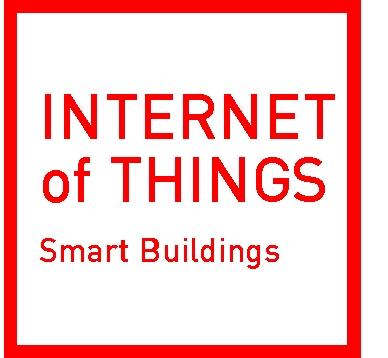
\includegraphics[width=0.26\linewidth]{iot-logo}
%	\begin{flushright}
%	
\includegraphics[width=0.4\linewidth]{TU_Logo_lang_RGB_schwarz}
%	\end{flushright}
		
\includegraphics[width=0.28\linewidth]{TU_Logo_lang_RGB_schwarz}
\hfill
			
\includegraphics[width=0.15\textwidth]{ecdf_logo}
			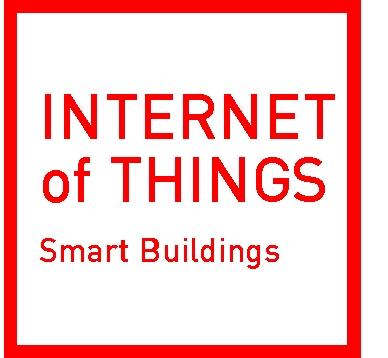
\includegraphics[trim=.05cm 0cm .47cm 0cm, clip, width=0.15\textwidth]{iot-logo}
	%
\includegraphics[width=0.42\linewidth]{TU_Logo_lang_RGB_schwarz}
	%\end{center}
    \begin{center}
			\vspace{2mm}
      %\large Master Thesis IOTSB XXX % for numbering
    \vfill
      \Large\textbf{Master's Thesis}\\
             \normalsize IOT-MT 001 % for numbering
			\LARGE \\~\\
      \textbf{Model predictive climate control based on Gaussian processes}\\
    \vspace{\fill}
      \Large Maxinne Musterfrau\\
      \small Registration number: 1234567\\
       ~\\
       \today \\
		\vfill
		  \normalsize
			\begin{tabular}{rl}
				First Examiner: & Prof. Dr.-Ing. Sergio Lucia\tabularnewline
				Second Examiner: & Prof. Dr.-Ing. XXX \tabularnewline
                Advisor:   & Maxi Mustermann\tabularnewline
			\end{tabular}
    \vfill
      \small  \selectlanguage{english}
			Technische Universit\"at Berlin\\
			Einstein Center Digital Future\\
			%{Department of Electrical Engineering and Computer Science}\\
			%\large{Laboratory for}\\
			~\\
			{Chair of Internet of Things for Smart Buildings}\\
			%~\\
			%\large{Prof. Dr.-Ing. Sergio Lucia}\\
%			\vfill
%			
\includegraphics[width=0.2\textwidth]{ecdf_logo}
%			\hfill
%			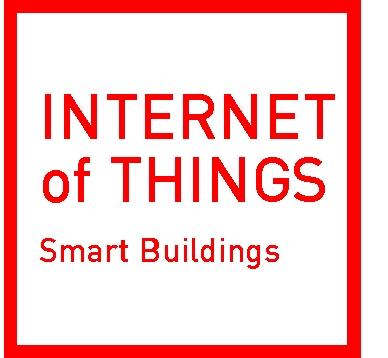
\includegraphics[trim=.05cm 0cm .47cm 0cm, clip, width=0.2\textwidth]{iot-logo}
		\end{center}
%    \begin{minipage}{0.2\linewidth}
%			\vspace{0.25cm}
%			
\includegraphics[width=0.95\textwidth]{ecdf_logo}
%			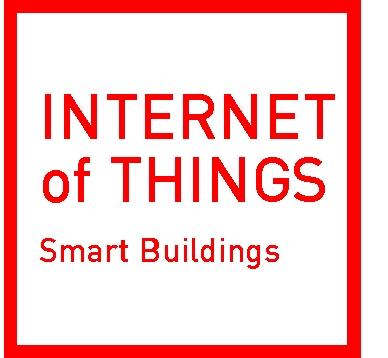
\includegraphics[trim=.05cm 0cm .47cm 0cm, clip, width=0.95\textwidth]{iot-logo}
%		\end{minipage}
%		\hfill
%		\begin{minipage}{0.79\linewidth}
%			\begin{flushright}
%			\large{Faculty for}\\
%			\large{Electrical Engineering and}\\
%			\large{Computer Science}\\
%			~\\
%			\large{Laboratory for}\\
%			\large{Internet of Things}\\
%			\large{for Smart Buildings}\\
%			~\\
%			\large{Prof. Dr.-Ing. Sergio Lucia}
%			\end{flushright}
%		\end{minipage}
\end{titlepage}
   % <-- Edit this one
\cleardoublepage              % next content starts on odd page


%% ABSTRACTS, TOC, etc. %%%%%%%%%%%%%%%%%%%%%%%%%%%%%%%%%%%%%%%%%%%%%%%
\pagenumbering{Roman}

\selectlanguage{english}
%%%%%%%%%%%%%%%%%%%%%%%%%%%%%%%%%%%%%%%%%%%%%%%%%%%%%%%%%%%%%%%%%%%%%%%%%%%%%%%%
%%%%%%%%%%%%%%%%%%%%%%%%%%%%%%%%%%%%%%%%%%%%%%%%%%%%%%%%%%%%%%%%%%%%%%%%%%%%%%%%
\addchap{Abstract}

The non-holonomic omnidirectional mobile robot has great potential in the industry market. The platform is equiped with 4 conventional centered wheels, and thus endued with large loading capability that is comparable with differential drive structures. In the mean time, the omnidirectional property makes it outperform differential drive structures in terms of flexibility. On the other hand, the holonomic omnidirectional counterparties has better maneuver flexibility. But the clastor or Swedish wheel they equipped can not hold large amount of loading and is more vulnerable to uneven ground. All these factors make non-holonomic omnidirectional structure a competitive candidate for industry use. 


However the control of this structure is still a complex task. This kind of robot only have 1 degree of mobility(DoF) which means they can not change their task space velocity instantly. Such constraint limit us from making full use of it's omnidirectional property. The existing solutions are focusing on pre-defined trajectory, but connected to navigation is a pre-request for it to be intelligent. Autonomous navigation for omnidirectional robot can generate trajectory that is inconsistent with time, especially for obstacle avoidance. Which is still a big challenge for the platform control.

The scope of this work is limited on the low-level controller, which takes the task space velocity/acceleration command as input, and output the joint reference signal to joint motors. Which assumes the existence of an omnidirectional global planner and a well-tuned motor dynamic controller.
%Since the augmented linear model predictive control scheme is linear the computational effort is comparable to conventional linear model predictive control.   % <-- Edit this one

% \selectlanguage{ngerman}
% %%%%%%%%%%%%%%%%%%%%%%%%%%%%%%%%%%%%%%%%%%%%%%%%%%%%%%%%%%%%%%%%%%%%%%%%%%%%%%%%
%%%%%%%%%%%%%%%%%%%%%%%%%%%%%%%%%%%%%%%%%%%%%%%%%%%%%%%%%%%%%%%%%%%%%%%%%%%%%%%%
\addchap{Deutsche Kurzfassung}

Die Regelung der Gebäudeklimatik hat zwei große Vorteile.
Erstens erlaubt sie das anpassen der Temperatur und der Luftfeuchtigkeit an die gewünschten Werte.
Dies kann beispielsweise in Bürogebäuden geschehen um angenehme Arbeitsbedingungen zu erzeugen oder in einem Gewächshaus um den Pflanzenwachstum zu maximieren.
Zweitens ermöglicht die Klimaregelung die Minimierung der Energieverbrauchs und -kosten.

Dabei ist das gleichzeitige Regeln eines Gebäudes und die Kostenminimierung schwer zu erreichen mit konventionellen Regelungsmethoden.
Modellprädiktive Regelung kann dieses Ziel erreichen aufgrund ihrer Fähigkeit Prädiktionen wie die Wettervorhersage in ihre Berechnungen einzubeziehen.
Desweiteren berücksichtigt modellprädiktive Regelung Bedingungen wie die Grenzwerte der Stellgrößen.

Mit nichtlinearer modellprädiktiver Regelung werden oft die besten Ergebnisse erzielt, weil die Klimadynamik nichtlinear und hochkomplex ist.
Da lineare modellprädiktive Regelung die nichtlinearen Anteile vernachlässigt ist ihre Genauigkeit geringer.
Die geringere Präzision vermindert die Kosteneinsparungen führt zu vermehrtem Verletzen der Bedingungen im Vergleich zu nichtlinearer modellprädiktiver Regelung.
Jedoch erfordert das nichtlineare Verfahren mehr Rechenleistung als das Lineare.
Desweiteren ist das Ableiten eines nichtlinearen Modells zeitaufwendig und erfordert weitreichende Fachkenntnisse.

Deshalb wird eine mit Gaußschen Prozessen erweiterte lineare modellprädiktive Regelung vorgestellt.
Die Gaußschen Prozesse werden verwendet um die vernachlässigten Nichtlinearitäten abzubilden und somit die Genaugkeit der Prädiktionen zu erhöhen im Vergleich zu konventioneller modellprädiktiver Regelung.
Die Gaußschen Prozesse werden als Parameter im linearen Prädiktionsmodell eingefügt.
Dadurch bleiben die Vorteile der linearen modellprädiktiven Reglung erhalten bei gleichzeitiger Verminderung der Nachteile.

In dieser Arbeit wurde gezeigt, dass die Kombination von linearer modellprädiktiver Regelung und Gaußschen Prozessen vergleichbare Ergebnisse erzielt bezüglich Kostenminimierung und Berücksichtigung der Bedingungen wie  nichtlineare modellprädiktive Regelung.
%Die erweiterte lineare modellprädiktive Regelung erfordert eine vergleichbare Rechenleistung wie konventionelle lineare modellprädiktive Regelung.   % <-- Edit this one
\cleardoublepage              % next content starts on odd page
%%%%%%%%%%%%%%%%%%%%%%%%%%%%%%%%%%%%%%%%%%%%%%%%%%%%%%%%%%%%%%%%%%%%%%%%%%%%%%%%
%%%%%%%%%%%%%%%%%%%%%%%%%%%%%%%%%%%%%%%%%%%%%%%%%%%%%%%%%%%%%%%%%%%%%%%%%%%%%%%%
\thispagestyle{empty}		% No header, footer, page number

\begin{center}
\LARGE{\textbf{Erklärung der Selbstständigkeit}}
\end{center}

\vspace{1cm} \noindent
Hiermit versichere ich, dass ich die vorliegende Arbeit
selbständig verfasst und keine anderen als die angegebenen Quellen und
Hilfsmittel benutzt habe.\\

\vspace{3em}
\begin{flushright}
	\begin{table}[ht]
		\begin{tabularx}{\textwidth}{Xp{4cm}}
      Magdeburg den \selectlanguage{ngerman} \today	& \\	
		\cline{2-2}
																	& \centering{Benjamin Karg}
		\end{tabularx}
	\end{table}
\end{flushright}
   % <-- Edit this one
\selectlanguage{english}
\tableofcontents

\addtocontents{toc}{\protect\vspace*{\baselineskip}}  % Add some space to the toc

\pagenumbering{arabic}


%% HERE COMES YOUR CONTENT %%%%%%%%%%%%%%%%%%%%%%%%%%%%%%%%%%%%%%%%%%%%
 \selectlanguage{english}    % uncomment if English is used throughout
                            % the whole document
\tikzset{
    wheelFrame/.pic={
		\draw[gray, very thick] (-0.8,-0.1) rectangle (0.8,0.1);
		\filldraw [gray] (0,0) circle (1pt);
		\draw[->] (0,0) -- (1,0) node[anchor=north west] {$x^{w#1}$};
		\draw[->] (0,0) -- (0,1) node[anchor=north west] {$y^{w#1}$}; 
	}
}
\tikzset{
    wheel/.pic={
		\draw[gray, very thick] (-0.8,-0.1) rectangle (0.8,0.1);
		\filldraw [gray] (0,0) circle (1pt);
	}
}
% \tikzset{
%     ICR/.pic={
		
% 		\filldraw [gray] (1.4,3.3) circle (1pt) node[\tikzpictextoptions]{\tikzpictext};
% 	}
% }
\tikzset{
    platform/.pic={
		\filldraw [gray] (0,0) circle (2pt);
			\draw[thick,->] (0,0) -- (5,0) node[anchor=north west] {$x^b$};
			\draw[thick,->] (0,0) -- (0,5) node[anchor=south east] {$y^b$};
			\draw[thick,->] (0.75,0) arc (0:90:0.75) node[anchor=south west] {$\theta^b$};
			\draw[black, thick] (-3,-3) rectangle (3,3);
	}
}
%%%%%%%%%%%%%%%%%%%%%%%%%%%%%%%%%%%%%%%%%%%%%%%%%%%%%%%%%%%%%%%%%
%2345678901234567890123456789012345678901234567890123456789012345
%        1         2         3         4         5         6     
\chapter{Introduction}
\label{cha:introduction}

Building climate control is a challenging task.
The climate of a building is highly complex and nonlinear system.
Using well-known approaches like PID controllers works well for single input single output (SISO) systems.
Whereas the implementation of PID controllers for multiple input multiple output (MIMO) systems like the building climate is tough.

Instead of using classical control approaches model predictive control (MPC) is applied.
MPC is designed to compute the optimal inputs for a MIMO system by predicting the future evolution of the system.
Moreover, MPC directly considers constraints like the limits of actuators.

Due to the nature of the climate the best results for building climate control are achieved using nonlinear prediction models.
One drawback of nonlinear MPC is the high computational expense compared to linear MPC as at every computation step a nonlinear optimization problem has to be solved instead of a linear.
Due to this fact linear MPC is easier to implement on micro-controllers which are usually very cheap and robust against environmental influences.
In warm and moist surroundings like inside a greenhouse installing an embedded system could be a proper solution.

However, using a linear prediction model to control a nonlinear process leads to neglecting the nonlinear dynamics.
Thus, the accuracy of linear MPC is lower than nonlinear MPC.

Hence, in this work a linear MPC scheme is presented which is extended with Gaussian processes (GP).
GPs are a machine-learning approach using stochastic methods to generate a function based on training data.
The GPs are used to estimate the error due to neglecting nonlinear dynamics using a linear prediction model.
Since the GPs are included in the prediction model as a precomputed parameter the optimal control problem stays linear.
Therefore, the new scheme provides a similar accuracy compared to nonlinear MPC while only requiring a computational expense compared to linear MPC.\par\medskip

%%%%%%%%%%%%%%%%%%%%%%%%%%%%%%%%%%%%%%%%%%%%%%%%%%%%%%%%%%%%%%%%%%%%%%%%%%%%%%%%%%%%%%%%%%%%%%%%%%%%%%%%%%%%%%%%%%%%%%%%%%%%%%%%%%%%%%%%%%%%%%%%%%%%%%%%%%%%%%%%%%%%%%%%%%%%%%%%%%%%%%%%%%%%%%%%%
%%%%%%%%%%%%%%%%%%%%%%%%%%%%%%%%%%%%%%%%%%%%%%%%%%%%%%%%%%%%%%%%%%%%%%%%%%%%%%%%%%%%%%%%%%%%%%%%%%%%%%%%%%%%%%%%%%%%%%%%%%%%%%%%%%%%%%%%%%%%%%%%%%%%%%%%%%%%%%%%%%%%%%%%%%%%%%%%%%%%%%%%%%%%%%%%%

This work focuses on two aspects to reach the above mentioned goals.
The first one is deriving an extended linear MPC scheme including GPs.
The works \cite{Kocijan.2003} and \cite{Kocijan.2004} present MPC based on GP prediction models.
The GPs are used for black-box identification of the real process and then included as prediction models.
However, in this work an existing linear model was augmented with GPs.

Works where existing models were extended are presented in \cite{Arahal.2005} and \cite{Klenske.2016}.
While in \cite{Arahal.2005} neuronal networks affecting the inputs are added to a finite impulse response model for simulating a greenhouse, in \cite{Klenske.2016} a GP is added to a linear model for predicting periodically occuring errors.
Since for both mentioned approaches of augmenting a linear model the extensions are directly included into the prediction model they are nonlinear MPC schemes.
Whereas, in this work the GPs are included as a precomputed parameter.
Therefore, the provided extended MPC scheme is linear.\par\medskip

The second aspect of the work regards building climate control which gained lot of attention in the recent years.
A survey is given by \cite{Cigler.2013} through describing the challenges of implementing building climate control.

An economic objective is defined for many approaches where MPC is used for climate control.
MPC approaches maximizing the energy efficiency of building climate control are \cite{Oldewurtel.2010} and \cite{Oldewurtel.2012} which are focusing on the weather forecast and \cite{Zhang.2013} which uses scenario-based MPC.
In this work the weather forecast is used for disturbance rejection in \cref{cha:setpoint} and in \cref{cha:economic} also for minimizing the cost of operating a building.
In \cite{Oldewurtel.2010b} real-time prices are considered to reduce the peak electricity demand, whereas in this work in \cref{cha:economic} the real-time prices for energy are considered to minimize the heating cost for a greenhouse.
%In \cite{Halvgaard.2012} applies economic MPC for building climate control in a smart grid.

Since in this work building climate control is shown using the example of a greenhouse following works were considered.
In \cite{RamirezArias.2005} was shown that MPC improves the efficiency of greenhouse heating systems which is important as heating is the main cost for operating a greenhouse.
Works describing a broad range of issues affecting the control of a greenhouse are \cite{Rodriguez.2015} and \cite{Bakker.1995}.\par\medskip

%%%%%%%%%%%%%%%%%%%%%%%%%%%%%%%%%%%%%%%%%%%%%%%%%%%%%%%%%%%%%%%%%%%%%%%%%%%%%%%%%%%%%%%%%%%%%%%%%%%%%%%%%%%%%%%%%%%%%%%%%%%%%%%%%%%%%%%%%%%%%%%%%%%%%%%%%%%%%%%%%%%%%%%%%%%%%%%%%%%%%%%%%%%%%%%%%
%%%%%%%%%%%%%%%%%%%%%%%%%%%%%%%%%%%%%%%%%%%%%%%%%%%%%%%%%%%%%%%%%%%%%%%%%%%%%%%%%%%%%%%%%%%%%%%%%%%%%%%%%%%%%%%%%%%%%%%%%%%%%%%%%%%%%%%%%%%%%%%%%%%%%%%%%%%%%%%%%%%%%%%%%%%%%%%%%%%%%%%%%%%%%%%%%

The first main contribution of this work is to provide an extended linear MPC scheme.
In comparison to conventional linear MPC the extended scheme includes in the prediction model a term estimating the error caused by the linearisation.
This error term is described by GPs and models the neglected nonlinear dynamics.

The second main contribution is the implementation of the provided MPC scheme in building climate control.
It is shown that the extended MPC scheme provides similar results compared to nonlinear MPC and outperforms conventional linear MPC.
This was verified for set-point tracking MPC of a greenhouse climate.
%Nonlinear MPC was defined as the benchmark since it used a perfect prediction model.
Moreover, applying the new scheme in economic MPC led to significant reductions of the operating costs compared to linear MPC.\par\medskip

%%%%%%%%%%%%%%%%%%%%%%%%%%%%%%%%%%%%%%%%%%%%%%%%%%%%%%%%%%%%%%%%%%%%%%%%%%%%%%%%%%%%%%%%%%%%%%%%%%%%%%%%%%%%%%%%%%%%%%%%%%%%%%%%%%%%%%%%%%%%%%%%%%%%%%%%%%%%%%%%%%%%%%%%%%%%%%%%%%%%%%%%%%%%%%%%%
%%%%%%%%%%%%%%%%%%%%%%%%%%%%%%%%%%%%%%%%%%%%%%%%%%%%%%%%%%%%%%%%%%%%%%%%%%%%%%%%%%%%%%%%%%%%%%%%%%%%%%%%%%%%%%%%%%%%%%%%%%%%%%%%%%%%%%%%%%%%%%%%%%%%%%%%%%%%%%%%%%%%%%%%%%%%%%%%%%%%%%%%%%%%%%%%%

The remainder of this thesis is organized as follows.
\cref{cha:greenhousemodel} discusses how to describe a greenhouse system based on (pseudo-) physical equations.
The MPC scheme is illustrated in \cref{cha:mpc} using the example of a linear discrete-time system.
In \cref{cha:gaussianprocesses} Gaussian Processes and their stochastic fundamentals are explained.
\cref{cha:implementation} describes how MPC and GPs are combined in a linear MPC scheme and which tools were used for the implementation.
In the following two chapters the results are discussed.
In both chapters the augmented MPC is compared to conventional linear MPC and nonlinear MPC.
At first, we take a look at the performance respective to set-point tracking in \cref{cha:setpoint}.
Afterwards, in \cref{cha:economic}, an economic MPC approach is analysed and the benefit of economic MPC over set-point tracking MPC is illustrated.
In \cref{cha:conclusion} the outcomes are put into conclusion and directions for future work are provided.   % <-- Edit this one
\chapter{Kinematic Model of Non-holonomic omnidirectional mobile robot}
\label{cha:Kinematic}





Kinematics is the most basic study of how mechanical systems behave. In our case, Kinematics make a connection between joint states(driving rate, steering angle and steering velocity) and platform velocity in the 
task space. Which is fundmental for our control method.
First, a overview of the mobile platform is given (\cref{sec:model_overview}).
Afterwards, the Forward and Inverse Kinematic equations (\cref{sec:hum}) are presented.
%\cref{sec:application} explains how the model is implemented in different model predictive control (MPC) approaches.

\section{Model overview}
\label{sec:model_overview}

The the platform is a regid squre body with four conventional wheels on each corner. each wheel can be controlled independently (steering/driving).

In the task space, the frame is as shown in \cref{fig:taskSpace} we use $ \xi = [x,t,\theta]$ to discribe the current platform position and orientation, use $ \dot{\xi} = [\dot{x},\dot{y},\dot{\theta}] $ and 
$ \ddot{\xi}= [\ddot{x},\ddot{y},\ddot{\theta}] $ to discribe the platform velocity and acceleration. 

In the following discussion, we will mainly focus on to frames, world frame in which the odometry $ \hat{\xi} $ is calculated, and body frame in which the platform velocity $\hat{\dot{\xi}}^b$ and platform 
acceleration $ \hat{\ddot{\xi}}^b $ is calculated, the command from global planer $ \dot{\xi}^b $ and $ \ddot{\xi}^b $ is also assumed to be in the body frame. The lower case "b" in the upper corner indicates 
this variable is expressed in the body frame. While the notion with "hat" like $\hat{}$ is used to expressed the measured feedback.


\begin{figure}[t]
	\begin{center}
	\resizebox{10cm}{!}
    {
		\begin{tikzpicture}[rotate=30 ]
			\pic[rotate=30 ] at(0,0) {platform};
			\pic[rotate=75 ] at(2.63,2.63) {wheelFrame};
			\pic[rotate=75 ] at(2.63,-2.63) {wheelFrame};
			\pic[rotate=75 ] at(-2.63,2.63) {wheelFrame};
			\pic[rotate=75 ] at(-2.63,-2.63) {wheelFrame};			
		\end{tikzpicture}
		}
	\end{center}
	\caption{Body frame and wheel frame}
\end{figure}





In the joint space we use $\beta_{i}$ and $\dot{\beta_{i}}$ to discribe the steering angle and steering velocity of the wheel, and $\dot{\phi}$ for driving velocity, which is shown in figure \cref{fig:wheel}. The measured
feedback from sensor is noted with $\hat{}$ while the joint space commands are without special notion. 






%%%%%%%%%%%%%%%%%%%%%%%%%%%%%%%%%%%%%%%%%%%%%%%%%%%%%%%%%%%%%%%%%%%%%%%%%%%%%
\section{Kinematics model}
\label{sec:Kinematics}
The Kinematic model is derived from the assumption that the wheels roll without slipping and there is no lateral skidding. The no-skidding constraint gurantee that there will be a unique instantaneous center of rotation(ICR) 
The ICR is term defined by Descartes' principle of instantaneous motion: 
\textit{At each instant, the motion of a planar rigid body coincides either with a pure translation, or with a pure rotation about some point, termed 
instantaneous center of rotation.}
Such feature distingushes this structure from the differential drive, gurantees the manuvior process to be quiet and robust.
We express the velocity of i-th wheel's contact point with ground by $V_{ci}=[v_{ti},v_{ni},0]$, where $v_{ti},v_{ni}$ respectively is the contact point's  tangential and normal velocitys. Which is illustrated in 
figure \cref{fig:contact_point}.



We can dirive the equation as follows:
\begin{equation}\label{eq:contact_point_velocity}
	\begin{split}
	V_{ci} &= T_b^{wi} [T_l^b\dot{\xi} + \dot{\theta}\overrightarrow{z_b}\times\overrightarrow{o_bo_{ci}} + \dot{\beta_i}T_{wi}^b\overrightarrow{z_{wi}}\times\overrightarrow{o_{wi}o_{ci}}] + \dot{\phi_i}\overrightarrow{x_{wi}}r_w
	\end{split}
\end{equation}

Where $T_b^w$,$T_l^b$ and $T_w^b$ are frame transfer matrix from body to wheel, from inertial to body and from wheel to body respectively. And $\overrightarrow{z_b}$, $\overrightarrow{z_w}$ and 
$\overrightarrow{x_w}$ are unit vectors along with positive direction of z axis of body frame, positive direction of z axis of wheel frame and positive direction of x axis of wheel frame.

With the above equation \cref{eq:contact_point_velocity} we can derive the contact point tangential velocity seprately
\begin{equation}\label{eq:contact_point_tangential}
	\begin{split}
	V_{ti} &= [cos(\beta_i), sin(\beta_i), -h_{yi}cos(\beta_i)+h_{xi}sin(\beta_i)]\dot{\xi^b} - r_w\dot{\phi_i}
	\end{split}
\end{equation}
And normal velocitys seprately.
\begin{equation}\label{eq:contact_point_normal}
	\begin{split}
	V_{ni} &= [-sin(\beta_i), cos(\beta_i), h_{xi}cos(\beta_i)+h_{yi}sin(\beta_i)]\xi^b
	\end{split}
\end{equation}

\subsection{Inverse Kinematics}
\label{sec:inverseKinematics}

To follow the constraints we defined in the begining, we set \cref{eq:contact_point_normal}$V_{ni}=0$. From which we can derive the expression of steering angles given the task space velocity command 
$\dot{\xi}=[\dot{x},\dot{y},\dot{\theta}]$.
\begin{equation}\label{eq:beta}
	\begin{split}
	\beta_i &= tan^{-1}(\frac{\dot{y^b}+h_{xi}\dot{\theta^b}}{\dot{x^b}-h_{yi}\dot{\theta^b}})
	\end{split}
\end{equation}

To express the steering velocity $\dot{\beta}$, we simplify the equation \cref{eq:contact_point_normal} by $V_{ni}=g(\dot{\beta_i})\dot{\xi^b}$ and differentiate it w.r.t. time:
\begin{equation}\label{eq:betaDot}
	\begin{split}
	\dot{\beta_i} &= \frac{-g(\dot{\beta_i})\ddot{\xi}}{\frac{dg(\dot{\beta_i})}{d\beta_i}\dot{\xi}}=\frac{\partial\beta_i}{\partial\dot{x}^b}\ddot{x}^b+\frac{\partial\beta_i}{\partial\dot{y}^b}\ddot{y}^b +\frac{\partial\beta_i}{\partial\dot{\theta^b}}\ddot{\theta}^b
	=f_{1i}(\dot{\xi^b})\ddot{\xi^b}
	\end{split}
\end{equation}

To express the driving rate of each wheel, we consider the constraint on tangential velocity, \cref{eq:contact_point_tangential} $V_{ti}=0 $ and we get:
\begin{equation}\label{eq:phi}
	\begin{split}
	\dot{\phi_i} &= \frac{1}{r_w}[cos(\beta_i), sin(\beta_i), -h_{yi}cos(\beta_i)+h_{xi}sin(\beta_i)]\dot{\xi^b}=f_{2i}(\beta)\dot{\xi^b}
	\end{split}
\end{equation}

Equation \cref{eq:beta},\cref{eq:betaDot} and \cref{eq:phi} illustrate the relationship between input velocity command in task space and the joint space response. By grouping them together, we get the Inverse Kinematics model


\subsection{Forward Kinematics}
\label{sec:forwardKinematics}

Similar to the process above, from \cref{eq:contact_point_tangential} we can also derive the forward Kinematic model, which takes the measured steering angle $\hat{\beta}$ driving velocity $\hat{\dot{\phi}}$ as input to 
calculate the platform current velocity $\hat{\dot{\xi}}$. For simplification, we simplify \cref{eq:contact_point_tangential}as $V_{fi}=f(\hat{\beta_i})\dot{\xi^b} -r_w\hat{\dot{\phi}}$
\begin{equation}
	\label{eq:forwardKinematics}
	\begin{split}
	\hat{\dot{\xi}} &= F^+(\hat{\beta})r_w\hat{\dot{\phi}},\\
	F(\hat{\beta}) &= [f(\hat{\beta_1})^T, f(\hat{\beta_2})^T, f(\hat{\beta_3})^T, f(\hat{\beta_4})^T]
	\end{split}
	\end{equation}
where $F^+(*)$ denotes pseudo inverse. One thing to be noticed is that classic psudo inverse will encountor singularities when platform has no rotation speed($\dot{\theta}=0$) where all 4 wheels are in parallel. In this case the $F(\hat{\beta})$matrix lose rank and the result would be inaccurate, we solve this by using the $pinv()$ function in Matlab and increase the singularity tolerance.

%%%%%%%%%%%%%%%%%%%%%%%%%%%%%%%%%%%%%%%%%%%%%%%%%%%%%%%%%%%%%%%%%%%%%%%%%%%%%%%%%%%%%%%%%%%%%%%%%%%%%%%%%%%%%%%%%%%%%%%%%%%%%%%%%%%%%%%%%%%%%%%%%%%%%%%%%%
%%%%%%%%%%%%%%%%%%%%%%%%%%%%%%%%%%%%%%%%%%%%%%%%%%%%%%%%%%%%%%%%%%%%%%%%%%%%%%%%%%%%%%%%%%%%%%%%%%%%%%%%%%%%%%%%%%%%%%%%%%%%%%%%%%%%%%%%%%%%%%%%%%%%%%%%%%


%%%%%%%%%%%%%%%%%%%%%%%%%%%%%%%%%%%%%%%%%%%%%%%%%%%%%%%%%%%%%%%%%
%2345678901234567890123456789012345678901234567890123456789012345
%        1         2         3         4         5         6     
\chapter{Mobile robot control framework}
\label{cha:framework}
A mobile robot is a complex system with several functional block. From control perspect of view, the system can be roughly divided into 2 parts, global planner and local planner.
Within this study we focus on the local planner which takes the task space velocity and acceleration command $\dot{\xi},\ddot{\xi}$ as input and calculate the corresponding optimal joint response, coordinate the steering and driving of four wheels, Which include 4 steering motors and 4 driving motors. The local planner communicate with these motors with CAN bus at 1 KHz, and take the task space command from global planner with ROS network at the same time.
The other part of the system is the global planner, which is responsible to sense the environment and make decision to plan the trajectory. It is out of scope of this paper, we just simplify it as a node which output task space command at 20Hz.


%%%%%%%%%%%%%%%%%%%%%%%%%%%%%%%%%%%%%%%%%%%%%%%%%%%%%%%%%%%%%%%%%%%%%%%%%%%%%%%%%%%%%%%%%%%%%%%%%%%%%%%%%%%%%%%%%%%%%%%%%%%%%%%%%%%%%%%%%%%%%%%%%%%%%%%%%%%%%%%%%%%%%%%%%%%%%%%%%%%%%%%%%%%%%%%%

\section{Structure}
\label{sec:structure}

\begin{figure}[t]
	\begin{center}
		\begin{tikzpicture}
		    \node (controller) at (0, 0) [rectangle, draw=red!50, text=red!70] {controller};
		    
			\node (steer1) at (2, 2.5) [rectangle, draw=black] {steer motor 1}
			edge [->, bend right] node[swap] {$\hat{\beta},\hat{\dot{\beta}}$} (controller)
			edge [<-] node[swap] {$\beta,\dot{\beta}$} (controller);
			
			\node (drive1) at (3, 2) [rectangle, draw=black] {drive motor 1}
			edge [->, bend left] node[swap] {$\dot{\phi}$} (controller)
			edge [<-] node[swap] {$\hat{\dot{\phi}}$} (controller);
			
			\node (steer2) at (2, -2.5) [rectangle, draw=black] {steer motor 2}
			edge [->, bend left] node[swap] {$\hat{\beta},\hat{\dot{\beta}}$} (controller)
			edge [<-] node[swap] {$\beta,\dot{\beta}$} (controller);
			
			\node (drive2) at (3, -2) [rectangle, draw=black] {drive motor 2}
			edge [->, bend right] node[swap] {$\dot{\phi}$} (controller)
			edge [<-] node[swap] {$\hat{\dot{\phi}}$} (controller);
			
			\node (steer3) at (-2, -2.5) [rectangle, draw=black] {steer motor 3}
			edge [post, bend right] node[swap] {$\hat{\beta},\hat{\dot{\beta}}$} (controller)
			edge [<-] node[swap] {$\beta,\dot{\beta}$} (controller);
			
			\node (drive3) at (-3, -2) [rectangle, draw=black] {drive motor 3}
			edge [->, bend left] node[swap] {$\dot{\phi}$} (controller)
			edge [<-] node[swap] {$\hat{\dot{\phi}}$} (controller);
			
			\node (steer4) at (-2, 2.5) [rectangle, draw=black] {steer motor 4}
			edge [->, bend left] node[swap] {$\hat{\beta},\hat{\dot{\beta}}$} (controller)
			edge [<-] node[swap] {$\beta,\dot{\beta}$} (controller);
			
			\node (drive4) at (-3, 2) [rectangle, draw=black] {drive motor 4}
			edge [->, bend right] node[swap] {$\dot{\phi}$} (controller)
			edge [<-] node[swap] {$\hat{\dot{\phi}}$} (controller);
		\end{tikzpicture}
	\end{center}
\end{figure}


%%%%%%%%%%%%%%%%%%%%%%%%%%%%%%%%%%%%%%%%%%%%%%%%%%%%%%%%%%%%%%%%%%%%%%%%%%%%%%%%%%%%%%%%%%%%%%%%%%%%%%%%%%%%%%%%%%%%%%%%%%%%%%%%%%%%%%%%%%%%%%%%%%%%%%%%%%%%%%%%%%%%%%%%%%%%%%%%%%%%%%%%%%%%%%%%

\section{Process model}
\label{sec:processmodel}

To guarantee a good performance of a MPC, the quality of the process model which is used for the predictions is crucial.
The model has to capture the major dynamics of the real controlled system otherwise the predicted states may deviate heavily from the real states.
Thus, the computed inputs may lead to constraint violations which render the control task infeasible.
To derive a process model, two general approaches can be considered.

The first one is first-principles modelling where the model is derived from physical laws.
The advantage of this method is that the parameters and their values have a meaning and the relations between the variables can be easily understood.
But it demands much knowledge in the specific field of application.

The second approach is system identification which can be generally divided into two groups.
In case of grey box system identification known relations and parameters are modelled while unknown ones are estimated via optimization with training data.
When black box system identification is applied, a strictly mathematical model with a certain amount of parameters is used, for example a neuronal network or a polynomial.

For all cases described above the obtained models have to be verified for different scenarios by comparing the real system with the process model.
The quality of the process model has to be optimized until it meets the requirements for a prediction model.
For more information about system identification see \cite{Isermann.2011} and \cite{Ljung.2012}.

The augmented MPC scheme presented in \cref{cha:implementation} relies on a linear continuous model:
\begin{equation}\label{eq:linss_cont}
\dot{\mathbf{x}}(t) = A\mathbf{x}(t)+B\mathbf{u}(t),
\end{equation}
where $\mathbf{x}(t)$ are states and $\mathbf{u}(t)$ are the inputs at time $t$.

However, since for solving the optimal control problem the continuous model is fully discretized at every time step $t_s$ using collocation our example system will be a linear discrete-time one described by:
\begin{equation}\label{eq:linss}
\mathbf{x}_{k+1}=A_{dis}\mathbf{x}_k+B_{dis}\mathbf{u}_k,
\end{equation}
where $\mathbf{x}_k$ are the states and $\mathbf{u}_k$ are the inputs at time step $k$.

%%%%%%%%%%%%%%%%%%%%%%%%%%%%%%%%%%%%%%%%%%%%%%%%%%%%%%%%%%%%%%%%%%%%%%%%%%%%%%%%%%%%%%%%%%%%%%%%%%%%%%%%%%%%%%%%%%%%%%%%%%%%%%%%%%%%%%%%%%%%%%%%%%%%%%%%%%%%%%%%%%%%%%%%%%%

\section{Prediction}
\label{sec:prediction}

If we want to predict the systems behaviour further than one step into the future, we have a function that is depending on future states.
In case of a prediction horizon of two time steps we can insert \eqref{eq:linss} in the first line of \eqref{eq:linpred2}.
\begin{align}\label{eq:linpred2}
\begin{split}
\mathbf{x}_{k+2} &= A_{dis} \mathbf{x}_{k+1} + B_{dis} \mathbf{u}_{k+1}, \\
                 &= A_{dis} \left(  A_{dis} \mathbf{x}_k + B_{dis} \mathbf{u}_k \right) + B_{dis} \mathbf{u}_{k+1}, \\
                 &= A_{dis}^2 \mathbf{x}_k + A_{dis} B_{dis} \mathbf{u}_k + B_{dis} \mathbf{u}_{k+1}.
\end{split}
\end{align}
Because the current state $\mathbf{x}_k$ and the current input $\mathbf{u}_k$ are known, $\mathbf{x}_{k+2}$ is only depending on $\mathbf{u}(T_s)$.
The same applies for predicting the state for all future time steps.
For the prediction of the states of the $n$-th future step at time step $k$ we get:
\begin{align}\label{eq:linpredn}
\begin{split}
\mathbf{x}_{k+n}&=A_{dis}^n\mathbf{x}_k+A_{dis}^{n-1}B_{dis}\mathbf{u}_k+\ldots\\
                &+A_{dis}B_{dis}\mathbf{u}_{k+n-2}+B_{dis}\mathbf{u}_{k+n-1}.
\end{split}
\end{align}
Thus, the future states are only a function of the current state $\mathbf{x}_k$ and the future inputs $\mathbf{u}_{k+i}$ which build the input trajectory.

%%%%%%%%%%%%%%%%%%%%%%%%%%%%%%%%%%%%%%%%%%%%%%%%%%%%%%%%%%%%%%%%%%%%%%%%%%%%%%%%%%%%%%%%%%%%%%%%%%%%%%%%%%%%%%%%%%%%%%%%%%%%%%%%%%%%%%%%%%%%%%%%%%%%%%%%%%%%%%%%%%%%%

\section{Objective function}
\label{sec:objective}

MPC is an optimal control approach with respect to the objective function.
The objective function describes the target of the control mathematically.
An example of a quadratic objective for the discrete-time state-space-model \eqref{eq:linss} is
\begin{equation}\label{eq:quadratic_cost}
J_{dis}(\mathbf{x},\mathbf{u}) = \sum_{k=1}^{n} (\mathbf{r}_k-\mathbf{x}_k)^TQ(\mathbf{r}_k-\mathbf{x}_k)+\mathbf{u}_k^TR\mathbf{u}_k,
\end{equation}
where $\mathbf{r}_k$ is the discrete reference trajectory, $n$ is the prediction horizon, $Q$ is the weighting matrix for states and $R$ is the weighting matrix for the inputs.
Large positive values in $Q$ result in a focus on sticking close to the reference trajectory while large positive values in $R$ enforce the minimization of used actuation energy.
To find the optimal input trajectory, the objective hast to be minimized while considering the constraints.

The resulting optimal control problem is described by:
\begin{subequations} \label{eq:description_conventional_mpc}
\begin{align}
\min \, J_{dis}(\mathbf{x},\mathbf{u})
\end{align}
subject to:
\begin{align}
\mathbf{x}_{k+1} = A\mathbf{x}_k+B\mathbf{u}_k,\\
\mathbf{x}_i \in \mathcal{X}, \mathbf{u}_i  \in \mathcal{U},\\
x_0 = x_{\text{init}},
\end{align}
\end{subequations}
where $\mathcal{X}$ and $\mathcal{U}$ are the compact and bounded spaces for feasible states and feasible inputs.

The state constraints are often implemented as box constraints.
Thus, they define the allowed maximum deviation from the reference trajectory.
The input constraints often describe the physical limits of the actuators.
As well the state constraints as the input constraints can be defined as soft and hard constraints.
The violation of hard constraints lead directly to an infeasible optimization problem, whereas the violation of soft constraints add a penalty term to the objective:
\begin{equation}\label{eq:soft}
J_{dis,soft}(\mathbf{x},\mathbf{u}) = J(\mathbf{x},\mathbf{u}) + \delta \sum_{k=1}^{n} \mathbf{v}_k,
\end{equation}
where $\delta$ is the weight of the penalty and $\mathbf{v}_k$ is the absolute value of the violation at time step $k$.

\eqref{eq:quadratic_cost} is a conventional objective function.
However, there are many approaches to design a economic objective function for minimizing the costs or maximizing the profit. 
A maximization problem can be easily transformed to a minimization problem by:
\begin{equation}\label{eq:minmaxJ}
\max \, J(\mathbf{x},\mathbf{u}) = \min \, -J(\mathbf{x},\mathbf{u}).
\end{equation}
In \cref{cha:economic} an approach to minimize the cost of operating a greenhouse is presented.

Since the models used in the following chapters are continuous the description of a continuous optimal control for \eqref{eq:linss_cont} given by:
%\begin{equation}\label{eq:description_conventional_mpc_cont}
%\begin{split}
%\min \, J_{cont}(\mathbf{x}(t),\mathbf{u}(t)) \quad s.t.\\
%\dot{\mathbf{x}}(t) = A\mathbf{x}(t)+B\mathbf{u}(t),\\
%\mathbf{x}(t) \in \mathcal{X}, \mathbf{u}(t)  \in \mathcal{U},\\
%\end{split}
%\end{equation}
\begin{subequations} \label{eq:description_conventional_mpc_cont}
\begin{align}
\min \, J_{cont}(\mathbf{x}(t),\mathbf{u}(t)) 
\end{align}
subject to:
\begin{align}
\dot{\mathbf{x}}(t) = A\mathbf{x}(t)+B\mathbf{u}(t),\\
\mathbf{x}(t) \in \mathcal{X}, \mathbf{u}(t)  \in \mathcal{U} \\
x_0 = x_{\text{init}},
\end{align}
\end{subequations}
where the objective function for the continuous case is described by:
\begin{equation}\label{eq:quadratic_cost_cont}
J_{cont}(\mathbf{x}(t),\mathbf{u}(t)) = \int_{0}^{t_f} \! (\mathbf{r}(t)-\mathbf{x}(t))^TQ(\mathbf{r}(t)-\mathbf{x}(t))+\mathbf{u}(t)^TR\mathbf{u}(t)\mathrm{d}t,
\end{equation}
where $\mathbf{r}(t)$ is the continuous reference trajectory and ${t_f}$ is the prediction horizon.

The relation between the prediction horizon of the continuous and the discrete-time is:
\begin{equation}\label{eq:rel_cont_dis}
t_f = n \cdot t_s.
\end{equation}
\par\medskip

In this chapter the model predictive control approach was explained.
Moreover, insight was given about prediction models, 
Thus, the first theoretical foundation of the expanded linear model predictive control scheme derived in \cref{cha:implementation} was presented.
In the following chapter GPs are presented which build the second theoretical foundation.


%%%%%%%%%%%%%%%%%%%%%%%%%%%%%%%%%%%%%%%%%%%%%%%%%%%%%%%%%%%%%%%%%
%2345678901234567890123456789012345678901234567890123456789012345
%        1         2         3         4         5         6     
\tdplotsetmaincoords{70}{110}     
\chapter{Approximation based Inverse Kinematic control}
\label{cha:inverseKinematics}
Due to the non-linear natural of the kinematic system, it is very hard to apply simple controllers on it. But as mentioned before, in some regions the kinematic system can be linearized without much error \cref{subsec:switching}. Based on such fact, we proposed a strategy that linearize the kinematic modle about the current platform state at each control instance by first order approximation. Thus we gain the linear system property and simply scale down the input of the system to limit the output joint space commands so that they don't violate acceleration limits.

%%%%%%%%%%%%%%%%%%%%%%%%%%%%%%%%%%%%%%%%%%%%%%%%%%%%%%%%%%%%%%%%%%%%%%%%%%%%%%%%%%%%%%%%%%%%%%%%%%%%%%%%%%%%%%%%%%%%%%%%%%%%%%%%%%%%%%%%%%%%%%%%%%%%%%%%%%%%%%%%%%%%%%%%%%%%%%%%%%%%%%%%%%%%%

\section{First order approximation}
\label{sec:firstOrderApp}
The kinematic equations used to calculate joint commands are \cref{eq:beta},\cref{eq:betaDot} and \cref{eq:phi}. As we are focusing on the acceleration limits rather than speed limits, \cref{eq:beta} is ignored here.

To distinguish the notions for different time step, we use $\dot{\xi}^n$ to indicate the current state of the platform, while $\dot{\xi}^{n-1},\dot{\xi}^{n+1}$ corresponding to the previous and next time step command.
Through Taylor Series expansions, we linearize \cref{eq:betaDot} and \cref{eq:phi} about the current platform status $\beta, \dot{\xi}^{n}$

\begin{equation}\label{eq:firstOrderApp}
\begin{split}
\dot{\beta}_i^{n+1}&=\dot{\beta}_i^n + \Delta\dot{\beta}_i=f_{1i}(\dot{\xi}^n)(\Delta\ddot{\xi}+\ddot{\xi}^n)\\
\dot{\phi}_i^{n+1}&=\dot{\phi}_i^n + \Delta\dot{\phi}_i=f_{2i}(\beta^n)(\Delta\dot{\xi}+\dot{\xi}^n)
\end{split}
\end{equation}
Assuming the acceleration applied during a control cycle is static, from the linearized approximation, we can extract the relationship between the joint jerk and task space command:
\begin{equation}\label{eq:deltaRelation}
    \begin{split}
        \ddot{\beta}^{n+1}&=\Delta\dot{\beta}_i/\Delta T=\frac{1}{\Delta T}f_{1i}(\dot{\xi}^n)\Delta\ddot{\xi}\\
        \ddot{\phi}^{n+1}&=\Delta\dot{\phi}_i/\Delta T=\frac{1}{\Delta T}f_{2i}(\beta^n)\Delta\dot{\xi}
    \end{split}
\end{equation}


\begin{figure}
    \centering
    \begin{tikzpicture}[scale=1.5,tdplot_main_coords]      
        \draw[thick,black,->] (0,0,0) -- (3,0,0) node[anchor=north east]{$x$};       
        \draw[thick,black,->] (0,0,0) -- (0,3,0) node[anchor=north west]{$y$};       
        \draw[thick,black,->] (0,0,0) -- (0,0,3) node[anchor=south]{$\theta$};        
        \draw[black,->] (0,0,0) -- (2,2,3) node[anchor=north west]{$\dot{\xi}^n$};
        \draw[black,->] (0,0,0) -- (3,1,2) node[anchor=north east]{$\dot{\xi}^{n+1}$};
        \draw[thick,blue,->] (2,2,3) -- (3,1,2) node[anchor= west]{$\Delta\dot{\xi}$};
\end{tikzpicture}
    \caption{Caption}
    \label{fig:deltaXi}
\end{figure}  

%%%%%%%%%%%%%%%%%%%%%%%%%%%%%%%%%%%%%%%%%%%%%%%%%%%%%%%%%%%%%%%%%%%%%%%%%%%%%%%%%%%%%%%%%%%%%%%%%%%%%%%%%%%%%%%%%%%%%%%%%%%%%%%%%%%%%%%%%%%%%%%%%%%%%%%%%%%%%%%%%%%%%%%%%%%%%%%%%%%%%%%%%%%%%%%%

\section{Covariance functions}
\label{sec:covfun}
For the way the knowledge is transferred from the training data to the Gaussian process model, the choice of the covariance function, more generally a kernel, is crucial.
A kernel is a mapping of a pair of inputs, $\mathbf{x} \in X$, $\mathbf{x}' \in X$ into $\mathbb{R}$.
By definition, a kernel has to be symmetric, that means $k(\mathbf{x},\mathbf{x}') = k(\mathbf{x}',\mathbf{x})$.
Given a set of test points $\mathbf{x}_i$, the Gram matrix $K$ with entries $K_{ij} = k(\mathbf{x}_i,\mathbf{x}_j)$ can be computed.
If the Gram matrix $K$ fulfills
\begin{equation}\label{eq:psd}
Q(\mathbf{v})=\mathbf{v}^T K \mathbf{v} \geq 0 \quad \forall \quad \mathbf{v} \in \mathbb{R}^n,
\end{equation}
it is positive semi-definite and therefore a covariance matrix. If additionally $Q(\mathbf{v})=0$ only when $\mathbf{v}=0$, $K$ is called positive definite and is also a covariance matrix.
If a covariance function is only a function of $\mathbf{x} - \mathbf{x'}$, it is called stationary. If it is only depending on $\left| \mathbf{x} - \mathbf{x'} \right|$, it is called isotropic. One example is the standard exponential kernel
\begin{equation}\label{eq:kse}
k_{SE}\left(\mathbf{x}, \mathbf{x}'\right)= \sigma_f^2 \cdot exp \left(-\frac{\left(\mathbf{x}-\mathbf{x}'\right)^2}{2l^2}\right),
\end{equation}
where $\sigma^2$ is highest possible correlation and $l$ is the lengthscale parameter.
It is possible to add and multiply different covariance functions to generate new ones.

%%%%%%%%%%%%%%%%%%%%%%%%%%%%%%%%%%%%%%%%%%%%%%%%%%%%%%%%%%%%%%%%%%%%%%%%%%%%%%%%%%%%%%%%%%%%%%%%%%%%%%%%%%%%%%%%%%%%%%%%%%%%%%%%%%%%%%%%%%%%%%%%%%%%%%%%%%%%%%%%%%%%%%%%%%%%%%%%%%%%%%%%%%%%%%%%

\section{Hyperparameters}
\label{sec:hyper}
Depending on the choice of the covariance function $k(\mathbf{x},\mathbf{x}')$, a set of hyperparameters $\theta$ has to be selected.
In case of the squared exponential kernel \ref{eq:kse} $\theta = \left\{\sigma_f^2,l\right\}$.
In most practical applications the majority of the hyperparameters are free, but sometimes fixing a hyperparameter makes sense.
For example if a periodic kernel should capture an effect related to the day-night-cycle, fixing its lengthscale to 24 hours seems appropriate.

\begin{figure}[t]
	\begin{subfigure}[b]{0.49\textwidth}
		\includegraphics[width=\textwidth]{../Figures/long.eps}
		\caption{$l = 2.0$}
		\label{fig:exl3}
	\end{subfigure}
	\hfill
	\begin{subfigure}[b]{0.49\textwidth}
		\includegraphics[width=\textwidth]{../Figures/short.eps}
		\caption{$l = 0.2$}
		\label{fig:exl4}
	\end{subfigure}
\caption{Impact of the hyperparameters on the predictions of a GP}
\label{fig:impact_lengthscale}
\end{figure}

To determine the optimal values of the free hyperparameters, the maximum likelihood estimation is used. Given the observations $x_1$, $x_2$,..., $x_n$ and the covariance function/statistical model $f(x)$, the joint density function for all observations is defined as
\begin{equation}\label{eq:jointdensity}
f(x_1,x_2,...,x_n)=f(x_1\mid\theta)\times f(x_2\mid\theta)\times...\times f(x_n\mid\theta).
\end{equation}
By looking at this equation from a new perspective, the likelihood
\begin{equation}\label{eq:likelihood}
\mathcal{L}(\theta;x_1,x_2,...,x_n)=f(x_,x_2,...,x_n\mid\theta)=\prod_{i=1}^nf(x_i\mid\theta)
\end{equation}
is a function of the hyperparameters $\theta$.
Therefore the observations $x_i$ are fixed parameters.
Thus, the optimal hyperparameters $\theta^*$ can be derived from  
\begin{equation}\label{eq:loglikelihood}
\theta^* = \underset{\theta}{\arg\max} \quad \mathcal{L}(\theta;x_1,x_2,...,x_n).
\end{equation}
In practice, often the natural logarithm is used because this simplifies the computation of the optimal hyperparameters while giving the same results.
\cref{fig:impact_lengthscale} shows the importance of the choice of the hyperparameters. A very short lengthscale leads to massive uncertainties of the predictions.\par\medskip

The previous sections explained what GPs are and how they are completely described by the mean function and covariance function.
Moreover, the optimization of the hyperparameters and their effect on the predictions were illustrated.

MPC and GP build the theoretical base for the augmented MPC scheme provided in this work.
The following chapter derives the augmented MPC by fusing predictive and learning-based control.
%%%%%%%%%%%%%%%%%%%%%%%%%%%%%%%%%%%%%%%%%%%%%%%%%%%%%%%%%%%%%%%%%
%2345678901234567890123456789012345678901234567890123456789012345
%        1         2         3         4         5         6     
\chapter{ICR optimization control}
\label{cha:ICR}
The implementation of the by GPs augmented MPC scheme is made up of three major steps.
First, MPC and GPs are conceptionally combined in an augmented MPC scheme in \cref{sec:augmentedcontroller}.
Second, a linear model for the prediction was derived in \cref{sec:predictionmodel}.
Third, in \cref{sec:software} the software used for the implementation is highlighted.

In this chapter the time-dependency is not explicitly written due to better readability.
%%%%%%%%%%%%%%%%%%%%%%%%%%%%%%%%%%%%%%%%%%%%%%%%%%%%%%%%%%%%%%%%%%%%%%%%%%%%%%%%%%%%%%%%%%%%%%%%%%%%%%%%%%%%%%%%%%%%%%%%%%%%%%%%%%%%%%%%%%%%%%%%%

\section{Augmented controller}
\label{sec:augmentedcontroller}
The purpose of the augmentation is to control a nonlinear process \eqref{eq:xdotnl} with a MPC scheme based on a linear prediction model \eqref{eq:xdotlin}.
\begin{align}
\dot{\mathbf{x}}_{nl} &= f \left( \mathbf{x},\mathbf{u},\mathbf{d} \right) \label{eq:xdotnl},\\
\dot{\mathbf{x}}_{lin} &= A \left( \mathbf{d} \right) \mathbf{x} + B \left( \mathbf{d} \right) \mathbf{u} + C \left( \mathbf{d} \right). \label{eq:xdotlin}
\end{align}
$\mathbf{x}$ denotes the states, $\mathbf{u}$ the inputs and $\mathbf{d}$ the disturbance variables which are treated as parameters.
The linear model is expanded with a term estimating the error $\mathbf{w}$:
\begin{align}
\dot{\mathbf{x}}_{aug} &= A \left( \mathbf{d} \right) \mathbf{x} + B \left( \mathbf{d} \right) \mathbf{u} + C \left( \mathbf{d} \right) + \mathbf{w}. \label{eq:xdotaug}
\end{align}
The error estimator $\mathbf{w}$ is described by a multidimensional Gaussian process
\begin{align}
\mathbf{w} \left(\mathbf{z}\right) \sim \mathcal{GP}\left( m \left(\mathbf{z} \right),k \left(\mathbf{z},\mathbf{z}' \right) \right),
\end{align}
where $\mathbf{z}$ is the concatenation of $\mathbf{x}$, $\mathbf{u}$ and $\mathbf{d}$.

The training data of the GPs is obtained by computing the error with \ref{eq:errorcomp} for a sufficient number of training points $\mathbf{z}_t$ of the input space.
\begin{align}
\mathbf{w} \left( \mathbf{z}_t \right) = \dot{\mathbf{x}}_{nl} \left( \mathbf{x}_t,\mathbf{u}_t,\mathbf{d}_t \right) - \dot{\mathbf{x}}_{lin} \left( \mathbf{x}_t,\mathbf{u}_t,\mathbf{d}_t \right). \label{eq:errorcomp}
\end{align}
After the GPs are optimized with the training data, they are added to the linear model.

In our concept two possible implementations are distinguished.
If the GP is linear, it is included directly into the optimization.
Otherwise it is treated as a parameter precomputed based on the predicted state and input trajectory of the previous optimization step and the known future disturbances.
This implementation is similar to a look-up table.
This distinction is done to keep the MPC scheme linear because of the advantageous presented in \cref{cha:introduction}.
The whole concept is depicted in \cref{fig:concept_controller}.

\begin{figure}[t]
\begin{center}
	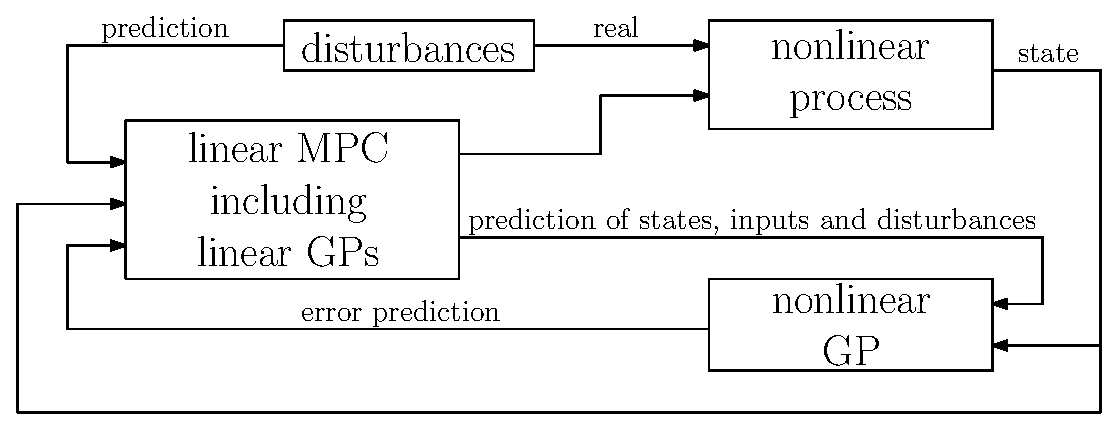
\includegraphics[width=\textwidth]{../Figures/concept_controller.eps}
	\caption{Concept of the augmented MPC}
	\label{fig:concept_controller}
\end{center}
\end{figure}

The full augmented MPC description is given by:
\begin{subequations}\label{eq:description_aug}
\begin{align}
\min \, &J(\mathbf{x},\mathbf{u};\mathbf{d},\mathbf{w})
\end{align}
subject to:
\begin{align}
\dot{\mathbf{x}}_{aug} = A \left( \mathbf{d} \right) \mathbf{x} &+ B \left( \mathbf{d} \right) \mathbf{u} + C \left( \mathbf{d} \right) + \mathbf{w},\label{eq:aug_dyn}\\
\mathbf{x} &\in \mathcal{X}, \mathbf{u} \in \mathcal{U},\label{eq:aug_sets}
\end{align}
\end{subequations}
and the optimal input trajectory $\mathbf{u}^*$ is obtained by:
\begin{align}
\mathbf{u}^* = \underset{\mathbf{u}}{\arg\min}~J(\mathbf{x},\mathbf{u};\mathbf{d},\mathbf{w}), \label{eq:uoptaug}
\end{align}
with respect to the constraints \eqref{eq:aug_dyn} and \eqref{eq:aug_sets}.

%%%%%%%%%%%%%%%%%%%%%%%%%%%%%%%%%%%%%%%%%%%%%%%%%%%%%%%%%%%%%%%%%%%%%%%%%%%%%%%%%%%%%%%%%%%%%%%%%%%%%%%%%%%%%%%%%%%%%%%%%%%%%%%%%%%%%%%%%%%%%%%%%

\section{Prediction model}
\label{sec:predictionmodel}
An analytical linearization of the nonlinear model described in \cref{cha:ICR} was used as the prediction model.
The nonlinear model is denoted as $f_{nl}(\mathbf{x},\mathbf{u};\mathbf{d})$.
The linearization at the point $(\mathbf{x}_0,\mathbf{u}_0)$ is described by:
\begin{align}
\begin{split}\label{eq:linearization}
f_{lin}(\mathbf{x},\mathbf{u};\mathbf{d}) &= f_{nl}(\mathbf{x}_0,\mathbf{u}_0;d)\\
                                          &+ \frac{\partial f_{nl}(\mathbf{x},\mathbf{u};\mathbf{d})}{\partial x} \bigg \vert_{\mathbf{x}_0,\mathbf{u}_0} \cdot (\mathbf{x} - \mathbf{x}_0)\\
                                          &+ \frac{\partial f_{nl}(\mathbf{x},\mathbf{u};\mathbf{d})}{\partial u} \bigg \vert_{\mathbf{x}_0,\mathbf{u}_0} \cdot (\mathbf{u} - \mathbf{u}_0).
\end{split}
\end{align}
\ref{eq:linearization} can also be expressed as a parameter-dependent state-space model \ref{eq:xdotlin}.
The parameters for the linearization are given in \cref{sec:lin_params}.

The linearisation is still parameter-dependent because of the bilinear properties of $f_{nl}(\mathbf{x}_0,\mathbf{u}_0;d)$.
Examining a simplified version of \ref{eq:beta}, described by:
\begin{equation}\label{eq:simple_rs}
Q_{rs,sim} = D_{rs,e}\cdot\left(1-U_{shd}\right),
\end{equation}
we can see that the magnitude of the effect of the shades $U_{shd}$ is heavily depending on the solar radiation $D_{rs,e}$. At night ($D_{rs,e} = 0$) the shades have no effect while at noon ($D_{rs,e} \approx \unit{800}{\nicefrac{W}{m^2}}$) they may be the only way to avoid too high temperatures. This is also the reason why prediction models derived from step and impulse responses perform badly when the environmental variables differ from the test scenario.

Another aspect of our prediction model is the error prediction with GPs.
Taking every variable into account would result in an input space with eleven dimensions.
To reduce the size of the GP identifying the major error sources is necessary.
The wind speed has a major effect on the greenhouse inside air temperature. Hence, establishing a GP for the wind speed $D_{ws,e}$ which is bilinearly and nonlinearly affected with opening percentage of the vents $U_{ven}$ results in an huge improvement of the linear model as \cref{cha:setpoint} will show.

\cref{fig:gp_optimization} shows the GP of the error of the temperature ODE.
Before the optimization of the hyperparameters the error seems arbitrary.
After the optimization a clear pattern is identifiable.
The greater the wind speed and the vents opening the greater the error.
Since the system is linearized around $(U_{ven} = 0.1, D_{ws,e} = 0)$ the error growth in dependence of the distance to this point seems valid.

% \begin{figure}[t]
% \begin{center}
% 	\begin{subfigure}[t]{.49\textwidth}
% 	\centering
% 		\includegraphics[width=\textwidth]{../Figures/gp_plot_not_opt.eps}
% 		\caption{Before optimization}
% 		\label{fig:gp_before_opt}
% 	\end{subfigure}
% 	\hfill
% 	%\newline
% 	\begin{subfigure}[t]{.49\textwidth}
% 	\centering
% 		\includegraphics[width=\textwidth]{../Figures/gp_plot_opt.eps}
% 		\caption{After optimization}
% 		\label{fig:gp_after_opt}
% 	\end{subfigure}
% \caption{GP describing the error for the temperature ODE caused by the linearization in dependence of $U_{ven}$ and $D_{ws}$}
% \label{fig:gp_optimization}
% \end{center}
% \end{figure}

%%%%%%%%%%%%%%%%%%%%%%%%%%%%%%%%%%%%%%%%%%%%%%%%%%%%%%%%%%%%%%%%%%%%%%%%%%%%%%%%%%%%%%%%%%%%%%%%%%%%%%%%%%%%%%%%%%%%%%%%%%%%%%%%%%%%%%%%%%%%%%%%%

\section{Software}
\label{sec:software}

The MPC was implemented via the use of several frameworks for Python 2.7.
\textbf{do-mpc} \cite{Lucia.2017}, a nonlinear MPC framework with integrated optimization, is the central element.
It consists of four modules: model, optimizer, observer and simulator.
Due to this modularity switching between different setups, e.g. changing the prediction model, is simple and analysis is simplified.

For the optimization tasks \textbf{Ipopt} \cite{Wachter.2006} is employed.
It is a primal-dual interior-point algorithm with a filter line-search method for nonlinear programming including second order corrections.
\textbf{CasADi} \cite{Andersson.01.01.2013} is a symbolic software tool for automatic differentiation and dynamic optimization used for the modeling and for the computation of first and second order derivative information.
\textbf{GPy} \cite{GPy.since2012} is the Gaussian process framework utilized for the augmented MPC. It includes a multitude of models, kernels and likelihoods for modelling stochastic processes and computing their optimal parameters.
\cref{fig:implementation_software} recaps the relations between the single software tools.
The module observer is not mentioned explicitly because full state feedback was used.\par\medskip

\begin{figure}[t]
\begin{center}
	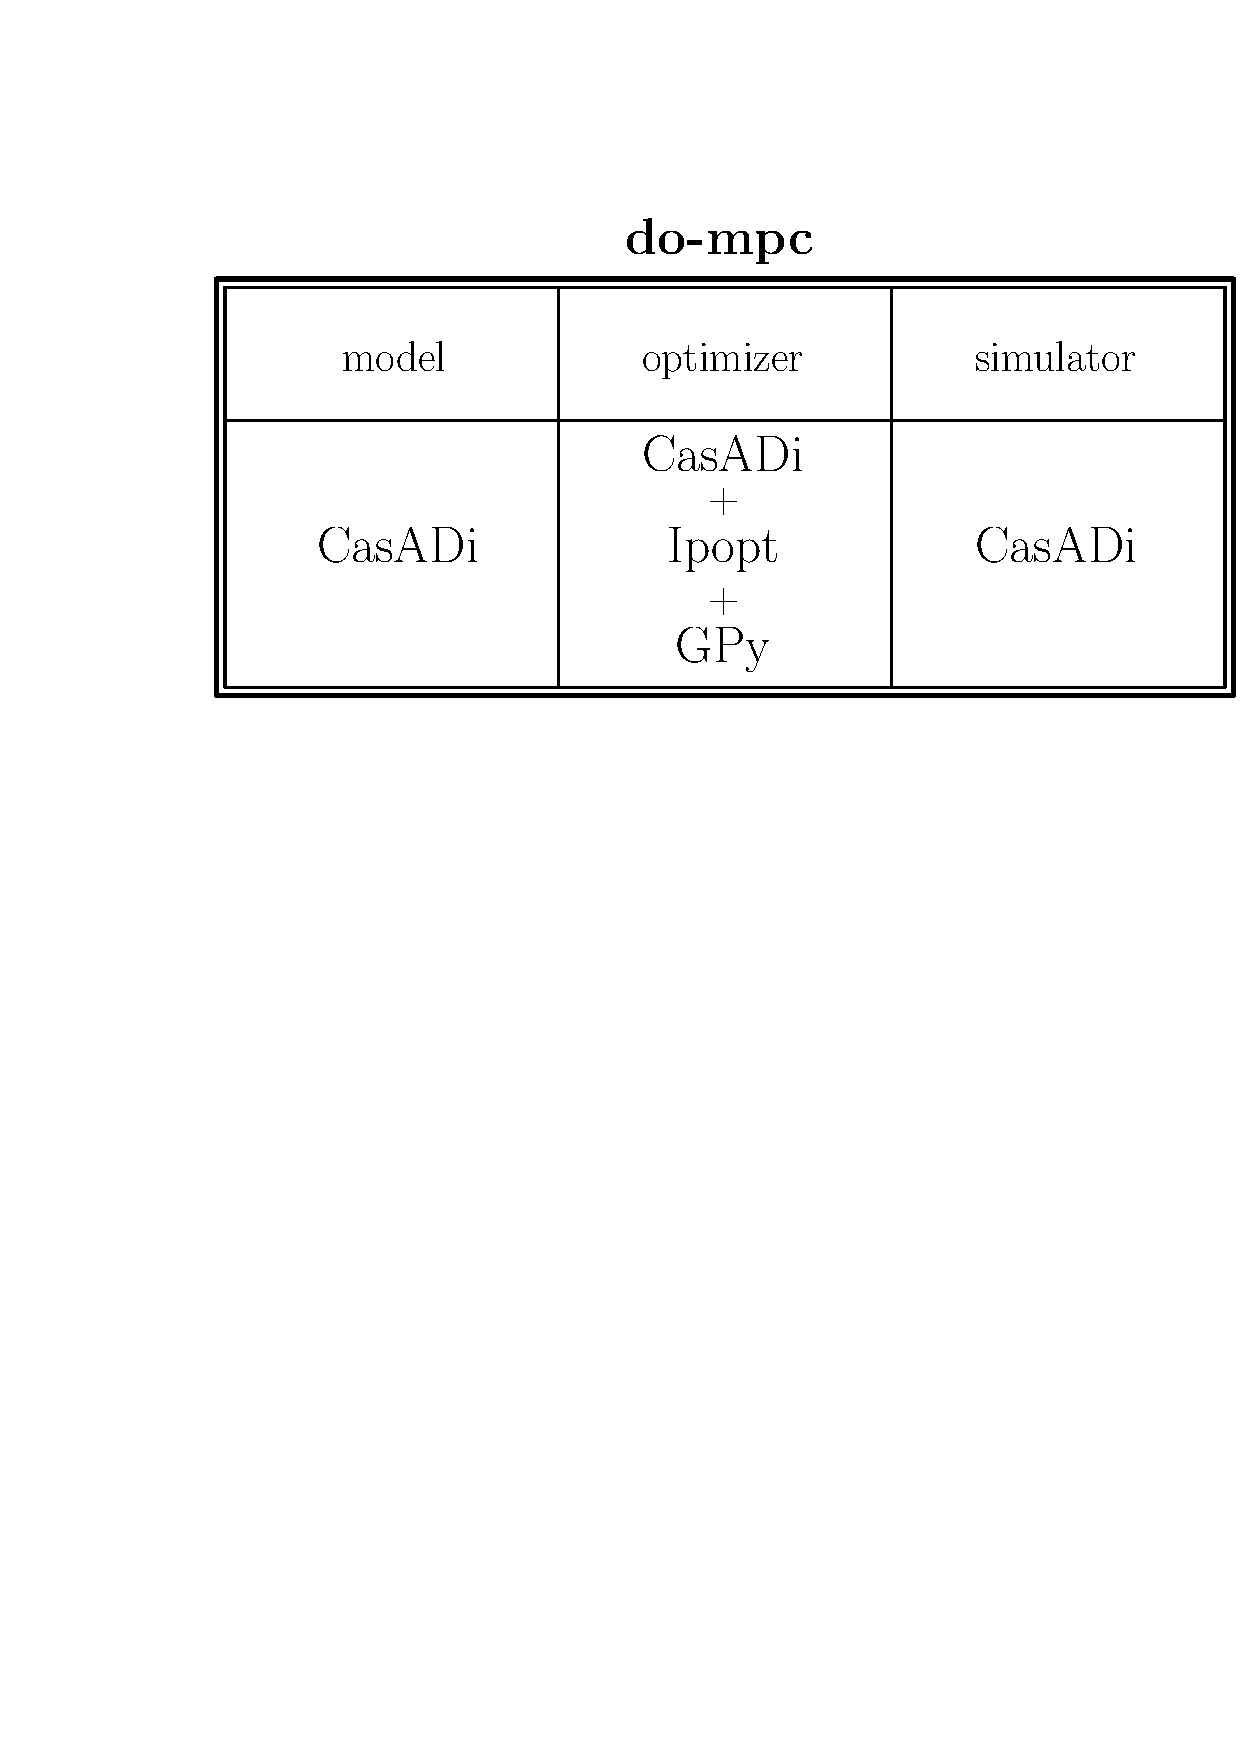
\includegraphics[width=\textwidth]{../Figures/implementation_software.pdf}
	\caption{Relations between the software tools}
	\label{fig:implementation_software}
\end{center}
\end{figure}

In summary, this chapter illustrated the concept of the expanded MPC approach.
Moreover, the linear prediction model used for the approach was derived and the software tools to implement the new concept were described.
In the following two chapters the newly derived augmented MPC scheme is used for set-point tracking (\cref{cha:setpoint}) and economic MPC (\cref{cha:economic}).
%%%%%%%%%%%%%%%%%%%%%%%%%%%%%%%%%%%%%%%%%%%%%%%%%%%%%%%%%%%%%%%%%
%2345678901234567890123456789012345678901234567890123456789012345
%        1         2         3         4         5         6     
\chapter{Experimental result}
\label{cha:experiment}
 The experiment is conducted both in simulation and ABB test prototype through collecting sensor feedback and apply forward kinematic on it.
The main design objective of our controller is it's performance under inconsistent task space command.

In this chapter we test 3 trajectories each represent a typical situation. 
\begin{itemize}
    \item[1] Pure rotation trajectory. From initial position, the platform makes a 360 degree rotation while the $\dot{x},\dot{y}$ remains 0 all the time.
    \item[2] 90 degree turn of heading. The task space velocity change from $\dot{\xi}=[1,0,0]$ to $\dot{\xi}=[0,1,0]$ in one control cycle.
    \item[3] Translation with rotation. Move 10 meters along x direction and rotate 360 degree simultaneously
\end{itemize}
The pure rotation trajectory require a sudden change of ICR position from infinite far away to origin, which corresponding to a 45 degree sudden change on steering angles. This most part of this trajectory will trigger the ICR control logic so it is used to test the ICR controller performance.

The 90 degree turn trajectory does not involve and angular velocity so the ICR is always infinite far away, thus only approximation based inverse kinematic control logic will be triggered. Thus this trajectory is used to test the performance of IKAM control logic.

The translation with rotation trajectory represents the general cases, where the task space command is generally smooth and ICR is changing position so that switching between 2 control logics happens frequently. Thus this trajectory is to test the general performance and the switching.
\begin{table}[!ht]
	\centering
		\begin{tabular}{cc}
		Trajectories   &  control strategy triggered                  \\\midrule
		Pure rotation          &  ICR, IKAM     \\
		90 degree turn          &  IKAM              \\
		Translation with rotation      &  ICR, IKAM              \\\bottomrule
		\end{tabular}
		\vspace{1mm}
	\caption{Nomenclature of the MPC approaches}
	\label{tab:testTrajectory}
\end{table}
This chapter is then divided by 4 sections, 3 of them explain 3 test trajectory and the last section discuss the advantage and problem we observe in the experiment.
%%%%%%%%%%%%%%%%%%%%%%%%%%%%%%%%%%%%%%%%%%%%%%%%%%%%%%%%%%%%%%%%%%%%%%%%%%%%%%%%%%%%%%%%%%%%%%%%%%%%%%%%
%%%%%%%%%%%%%%%%%%%%%%%%%%%%%%%%%%%%%%%%%%%%%%%%%%%%%%%%%%%%%%%%%%%%%%%%%%%%%%%%%%%%%%%%%%%%%%%%%%%%%%%%
\section{Pure rotation trajectory}
\label{sec:pureRotationTraj}
\subsection{Task space velocity performance}
For this trajectory, the reference command has no translation velocity, which means $\dot{x}_{ref}=0, \dot{y}_{ref}=0$ holds all the time. While the $\dot{\theta}_{ref}$ is a function of time which is illustrate in \cref{fig:PR_t} as reference signal. The controller generated response $\dot{x}_{hat}$ is also shown in the figure, and we can see that it takes around 1 second for the platform to do the initialization, and after that the wheel is oriented to the desired position, and the reference command is perfectly followed.
\begin{figure}[!h]
    \centering
    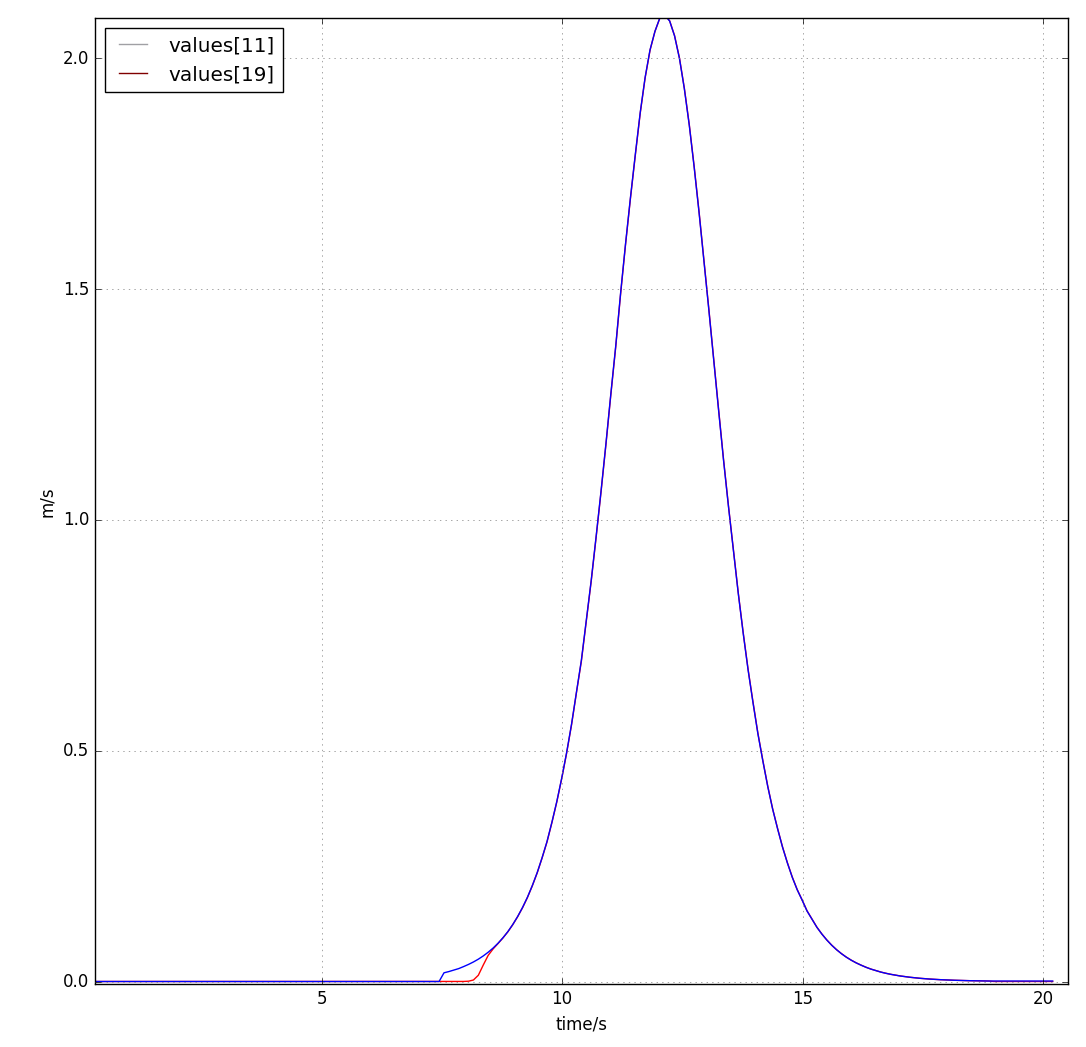
\includegraphics[width=0.6\textwidth]{Figures/PR_t.png}  
    \caption{Reference command and response on $\dot{\theta}$}
    \label{fig:PR_t}
\end{figure}

Then we look into the $\dot{x}$ and $\dot{y}$ performance in \cref{fig:PRtranslation}, we can see that even though the reference command remains 0 for both direction, the generated response still have a small velocity on $\dot{x}$ direction in \cref{fig:PRtranslationX}. That is due to the fact that the initial wheel orientation cannot conduct pure rotation command, this is constrained by the DoM. And the intermediate $\Tilde{\dot{\xi}}_{ref}$ generated by ICR control logic will contain a small component on x direction to make $\Tilde{\dot{\xi}}_{ref}$ respect kinematic constraint. The small disturbance between $t=10-20s$ is caused by accuracy issue of optimization algorithm.
\begin{figure}[!hb]
     \centering
     \begin{subfigure}[b]{0.49\textwidth}
         \centering
          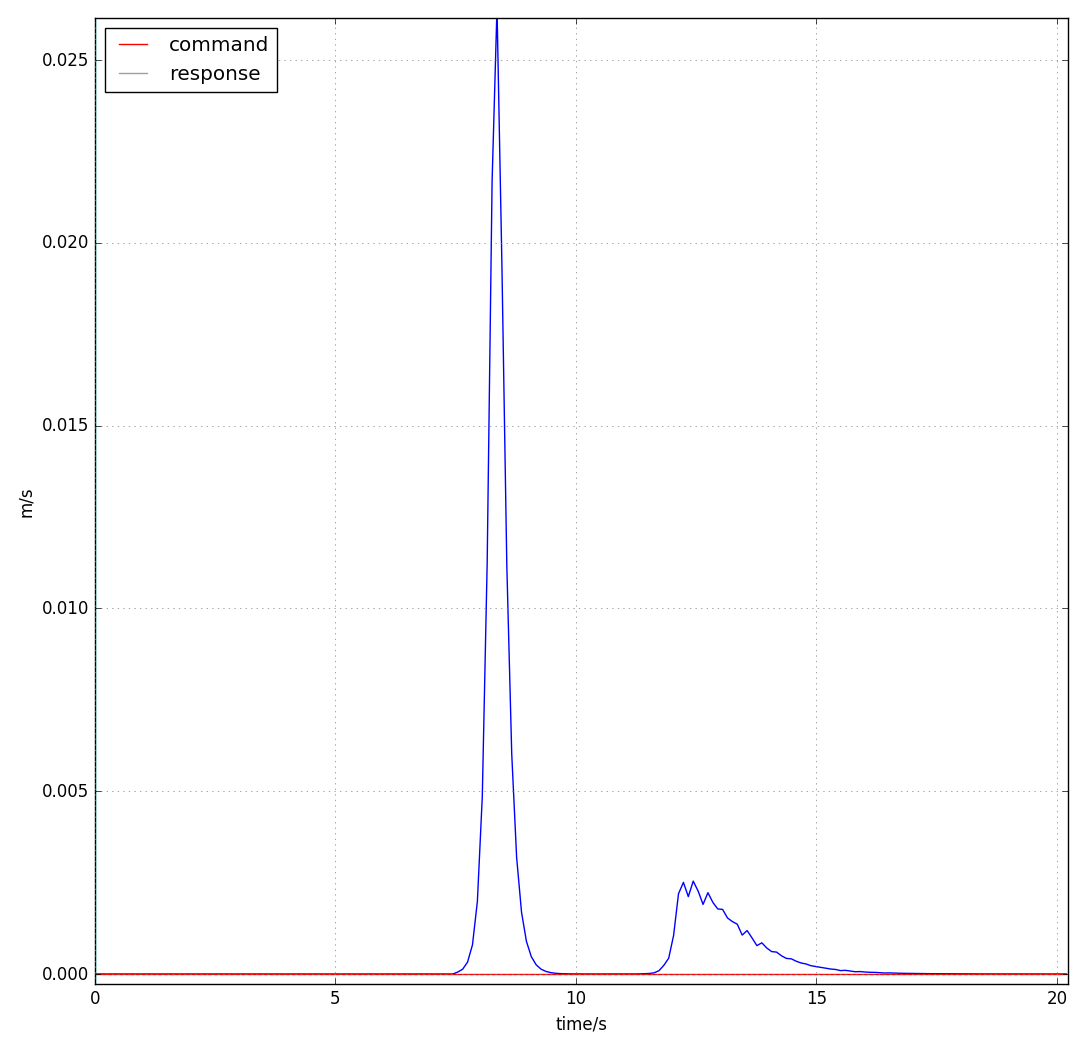
\includegraphics[width=1.2\textwidth]{Figures/PR_x.png}
         \caption{$\dot{x}$}
         \label{fig:PRtranslationX}
     \end{subfigure}
     \hfill
     \begin{subfigure}[b]{0.49\textwidth}
         \centering
         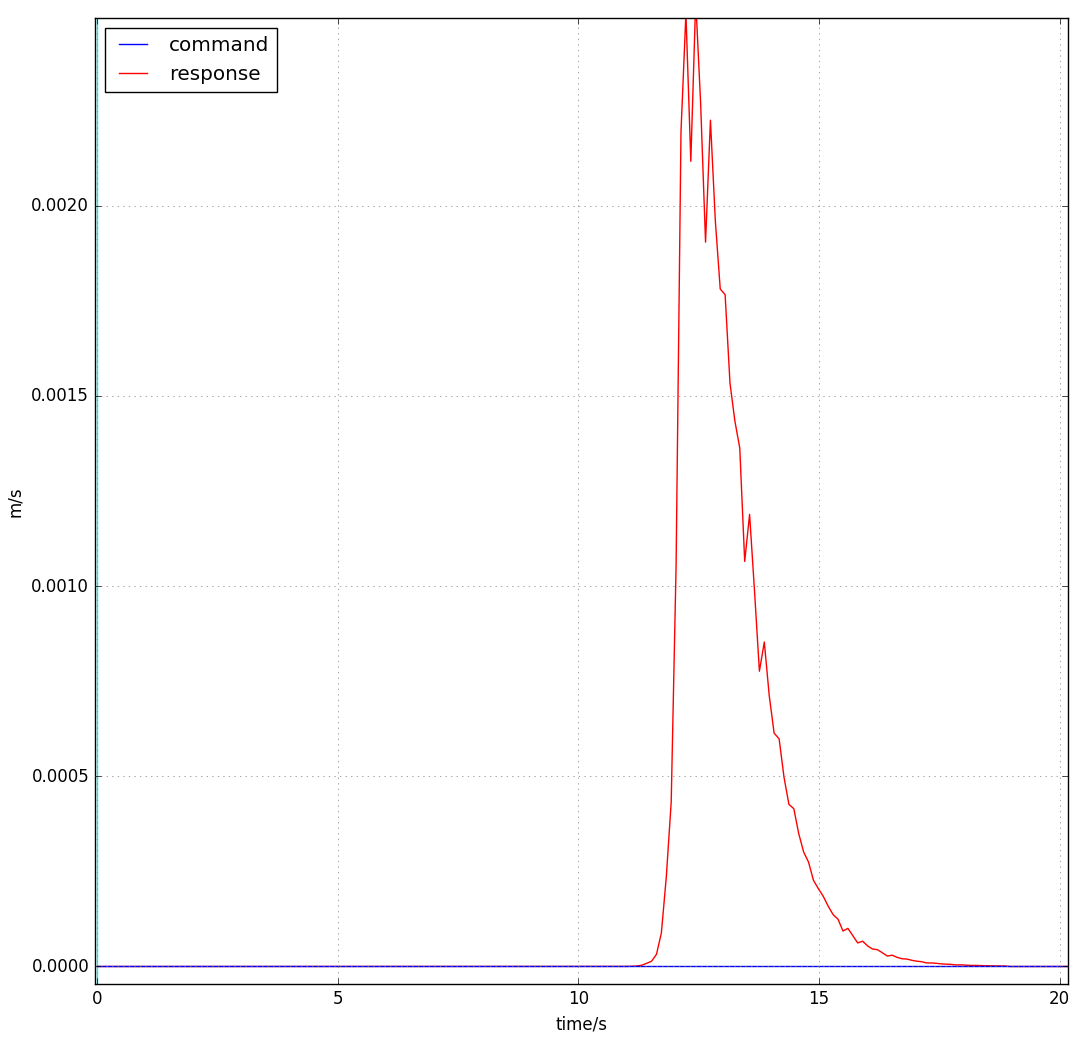
\includegraphics[width=1.2\textwidth]{Figures/PR_y.png}
         \caption{$\dot{y}$}
         \label{fig:PRtranslationY}
     \end{subfigure}
     
        \caption{translation velocity}
        \label{fig:PRtranslation}
\end{figure}
%%%%%%%%%%%%%%%%%%%%%%%%%%%%%%%%%%%%%%%%%%%%%%%%%%%%%%%%%%%%%%%%%%%%%%%%%%%%%%%%%%%%%%%%%%%%%%%%%%%%%%%%
\subsection{ICR response}
Our controller directly manipulate on ICR, so the output $ICR_{next}$ contain a lot of information of the controller behavior. As shown in \cref{fig:PR_ICRx}, the x component of reference ICR keeps 0 along the trajectory, but due to constraint and optimization accuracy issue, the executed $ICR_{next}$ is slightly deviated from 0. And if we look at \cref{fig:PR_ICRy}, the y component of $ICR_{ref}$ also keeps 0 along the trajectory. The control logic switch to ICR control at time $t=3.5$ and the response y component of $ICR_{next}$ start from a very large value, and smoothly move to the desired value. The whole process takes less than 1 second.
\begin{figure}[!h]
    \centering
    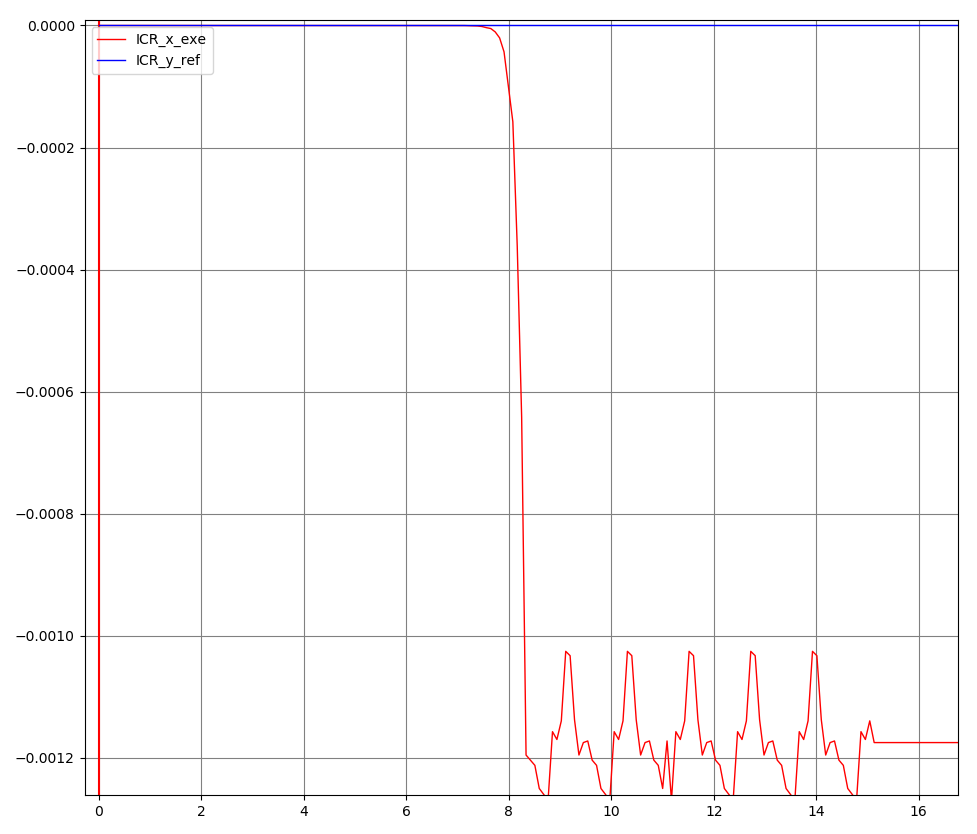
\includegraphics[width=\textwidth]{Figures/PR_ICR_x.png}
    \caption{$\Tilde{ICR_x}$ }
    \label{fig:PR_ICRx}
\end{figure}

\begin{figure}[!h]
    \centering
    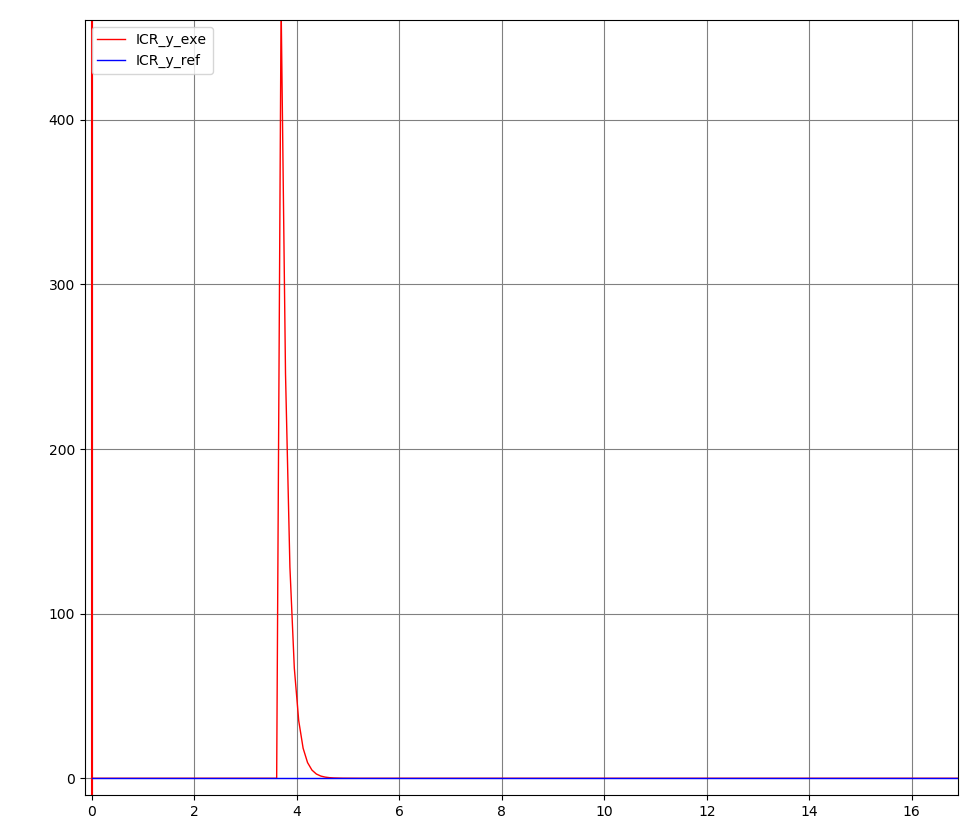
\includegraphics[width=1\textwidth]{Figures/PR_ICR_y.png}
    \caption{$\Tilde{ICR_y}$ }
    \label{fig:PR_ICRy}
\end{figure}
%%%%%%%%%%%%%%%%%%%%%%%%%%%%%%%%%%%%%%%%%%%%%%%%%%%%%%%%%%%%%%%%%%%%%%%%%%%%%%%%%%%%%%%%%%%%%%%%%%%%%%%%
%%%%%%%%%%%%%%%%%%%%%%%%%%%%%%%%%%%%%%%%%%%%%%%%%%%%%%%%%%%%%%%%%%%%%%%%%%%%%%%%%%%%%%%%%%%%%%%%%%%%%%%%
\section{Turning 90 degree}
\label{sec:90degree}
Through out this trajectory, $\dot{\xi}_{ref}$ changes from $[1,0,0]$ to $[0,1,0]$ and end up with $[-1,0,0]$. Appears to be 90 degree turning of heading for 2 times. While the $\dot{\theta}$ component of $\dot{\xi}_{ref}$ keeps being 0, which means no rotation involved in the trajectory.

The ICR keeps being infinite far away through out the trajectory, the ICR control logic will not be triggered. And the Approximation based control logic is examined. The performance on x and y direction is shown in \cref{fig:90}. The trajectory has 3 inconsistency points, at time $t=4$ the reference signal changes from $\dot{\xi}=[0,0,0]$ to $\dot{\xi}=[1,0,0]$, no steering angle change is needed here as $\dot{\xi}=[1,0,0]$ require the same steering angle as the initial state. So that we can see the response of wheel almost perfectly match the reference.

At $t=8$ reference changes to $\dot{\xi}=[0,1,0]$, here a 90 degree sudden change of steering angle is needed and we can see that the it takes around 1 second for the intermediate reference $\dot{\xi}$ to reach the target.

And at $t=12.2$ the reference end up with $\dot{\xi}=[-1,0,0]$. the behavior is similar as before.  The reference signal in the figure is what we used to give motor command, but the motor control it self is not with in our scope. One thing to be noticed is that the steer motors have slight overshot for this trajectory.
\begin{figure}[!hb]
     \centering
     \begin{subfigure}[b]{0.49\textwidth}
         \centering
          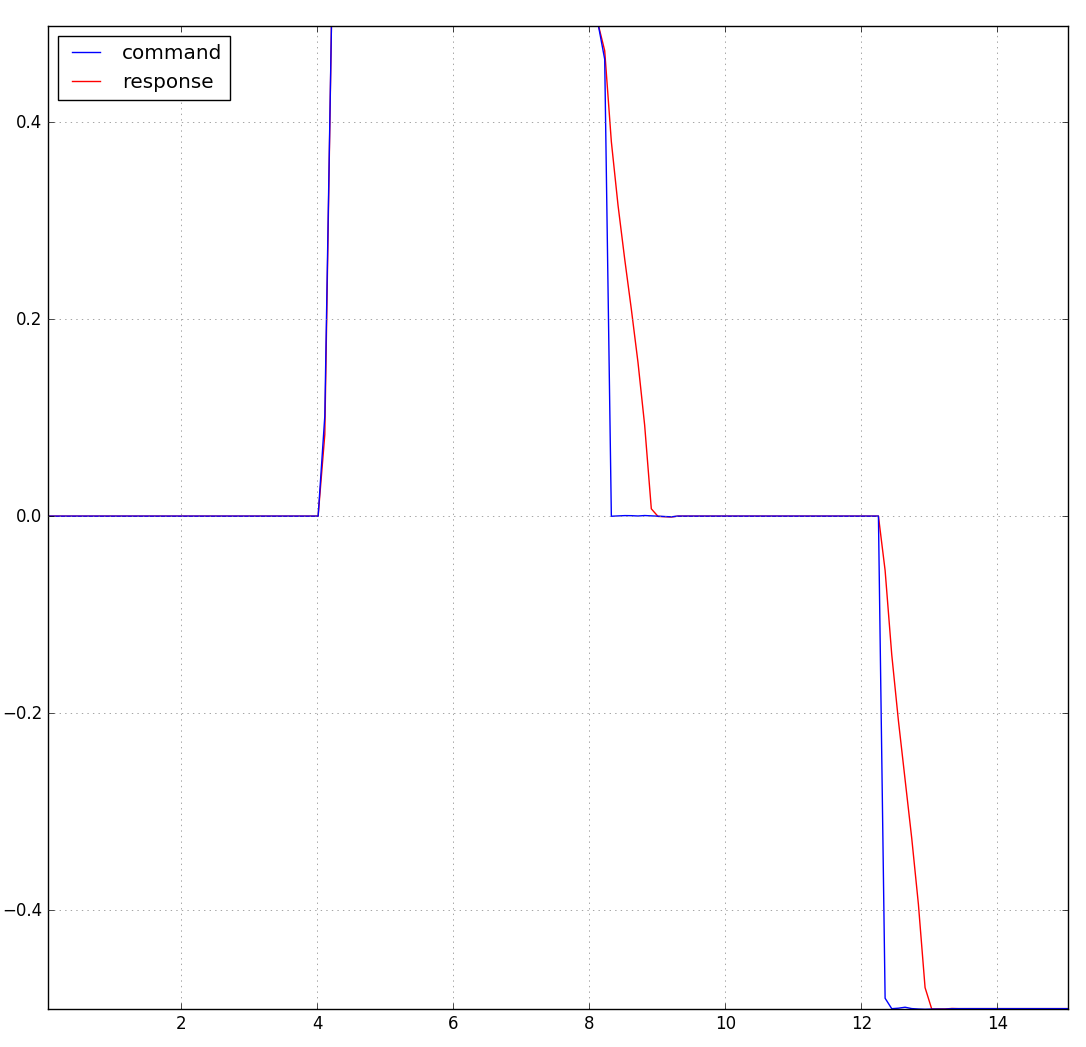
\includegraphics[width=1.1\textwidth]{Figures/90_x.png}
         \caption{$\dot{x}$}
         \label{fig:90X}
     \end{subfigure}
     \hfill
     \begin{subfigure}[b]{0.49\textwidth}
         \centering
         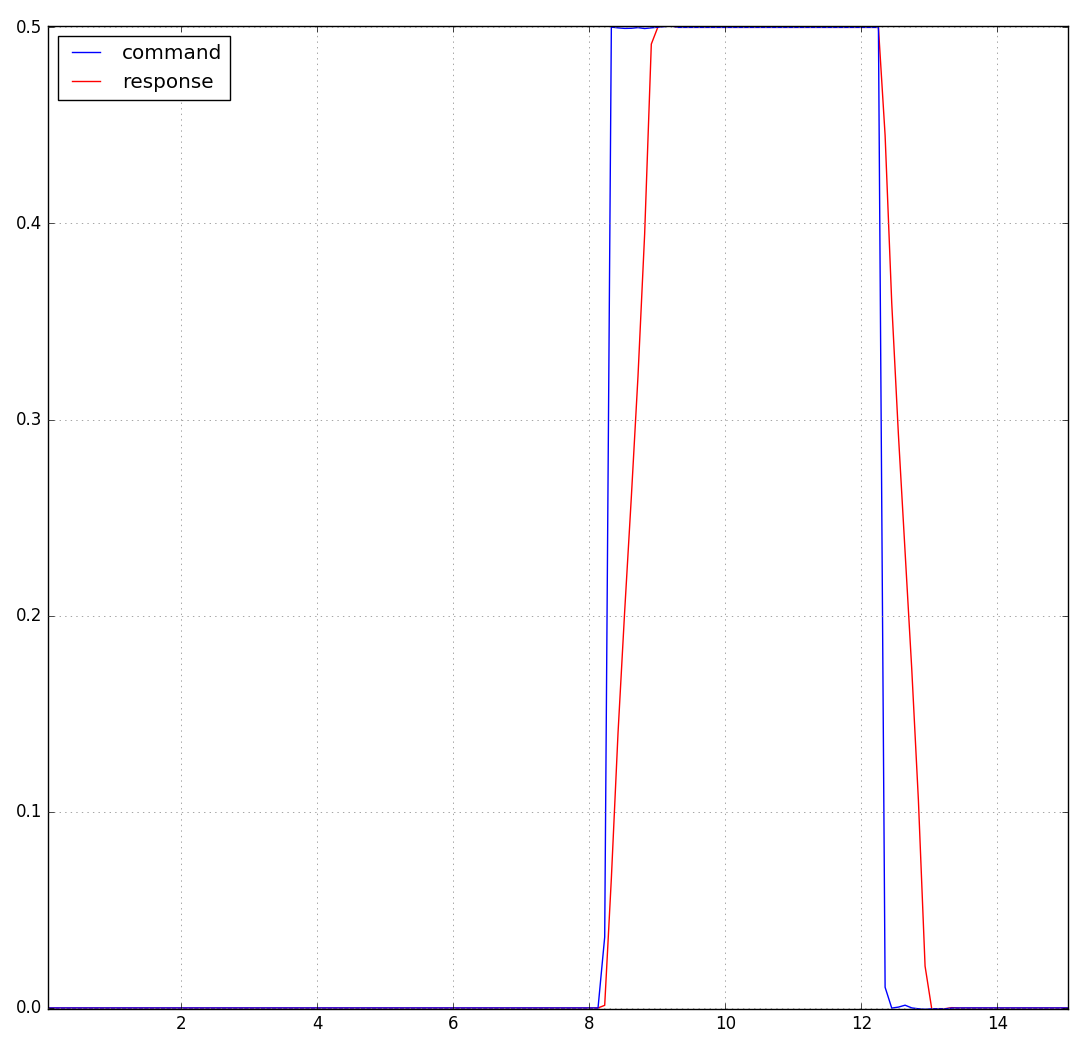
\includegraphics[width=1.1\textwidth]{Figures/90_y.png}
         \caption{$\dot{y}$}
         \label{fig:90Y}
     \end{subfigure}
     
        \caption{translation velocity}
        \label{fig:90}
\end{figure}
% \begin{figure}[!ht]
%     \centering
%     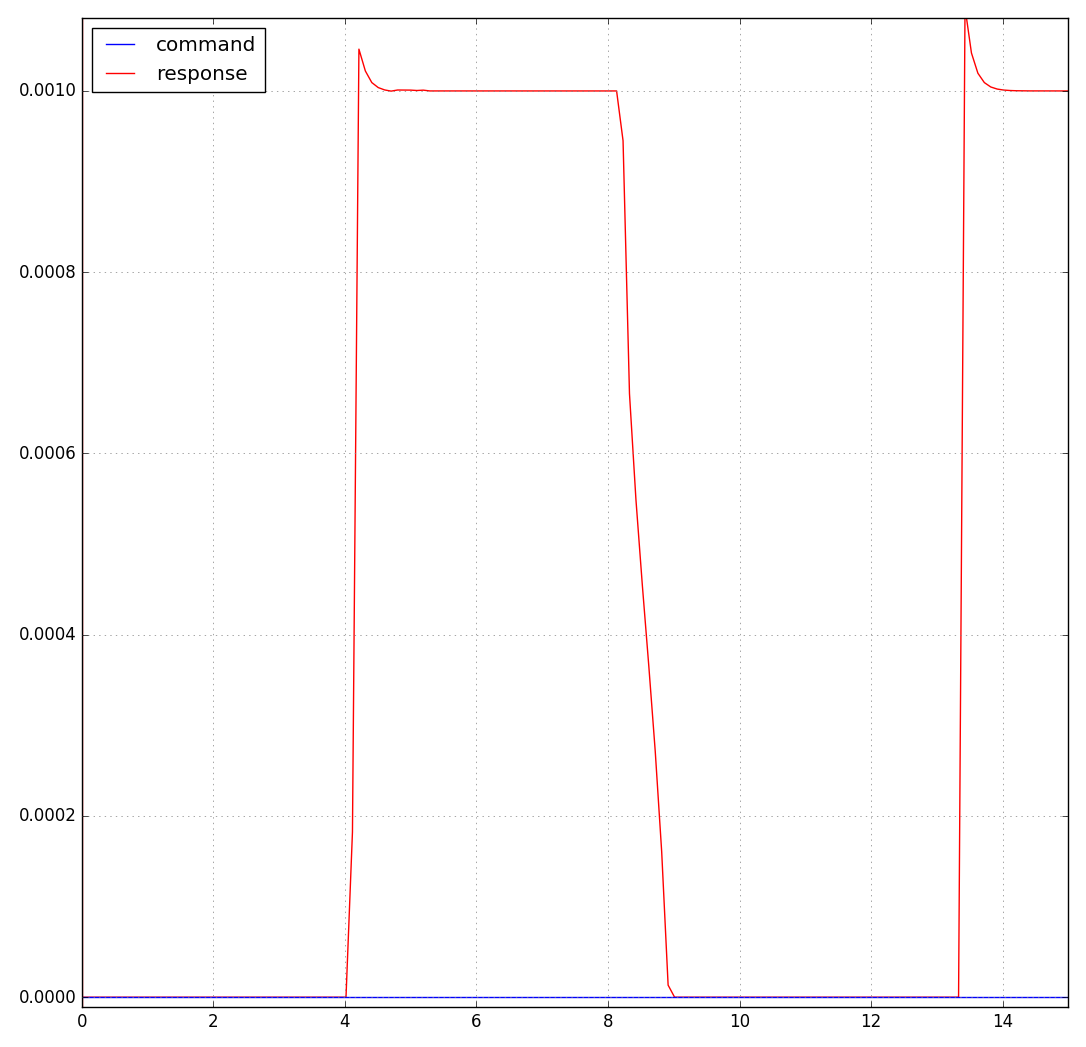
\includegraphics[width=0.7\textwidth]{Figures/90_t.png}
%     \caption{Caption}
%     \label{fig:my_label}
% \end{figure}

% \begin{figure}[!h]
%     \centering
%     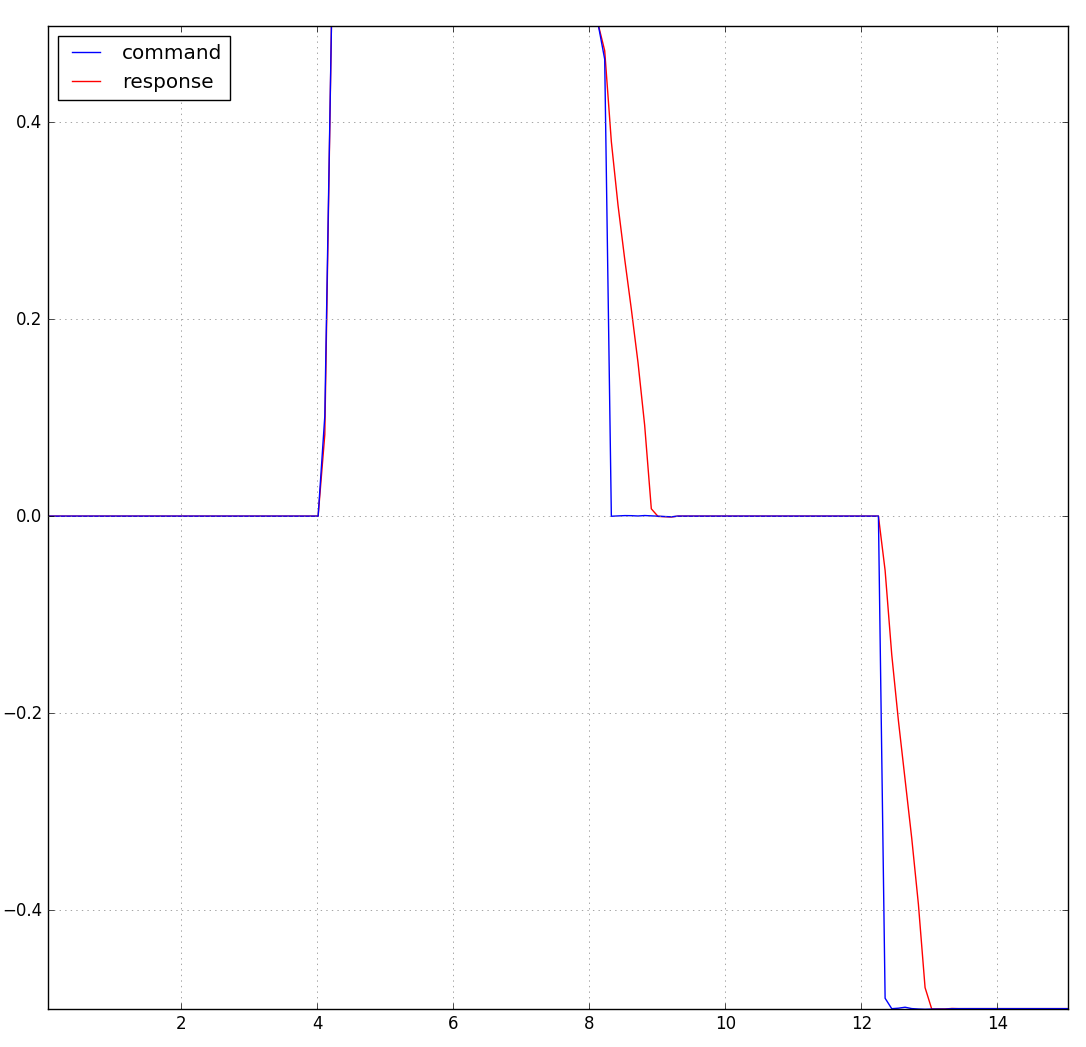
\includegraphics[width=0.7\textwidth]{Figures/90_x.png}
%     \caption{Caption}
%     \label{fig:my_label}
% \end{figure}
% \begin{figure}[!h]
%     \centering
%     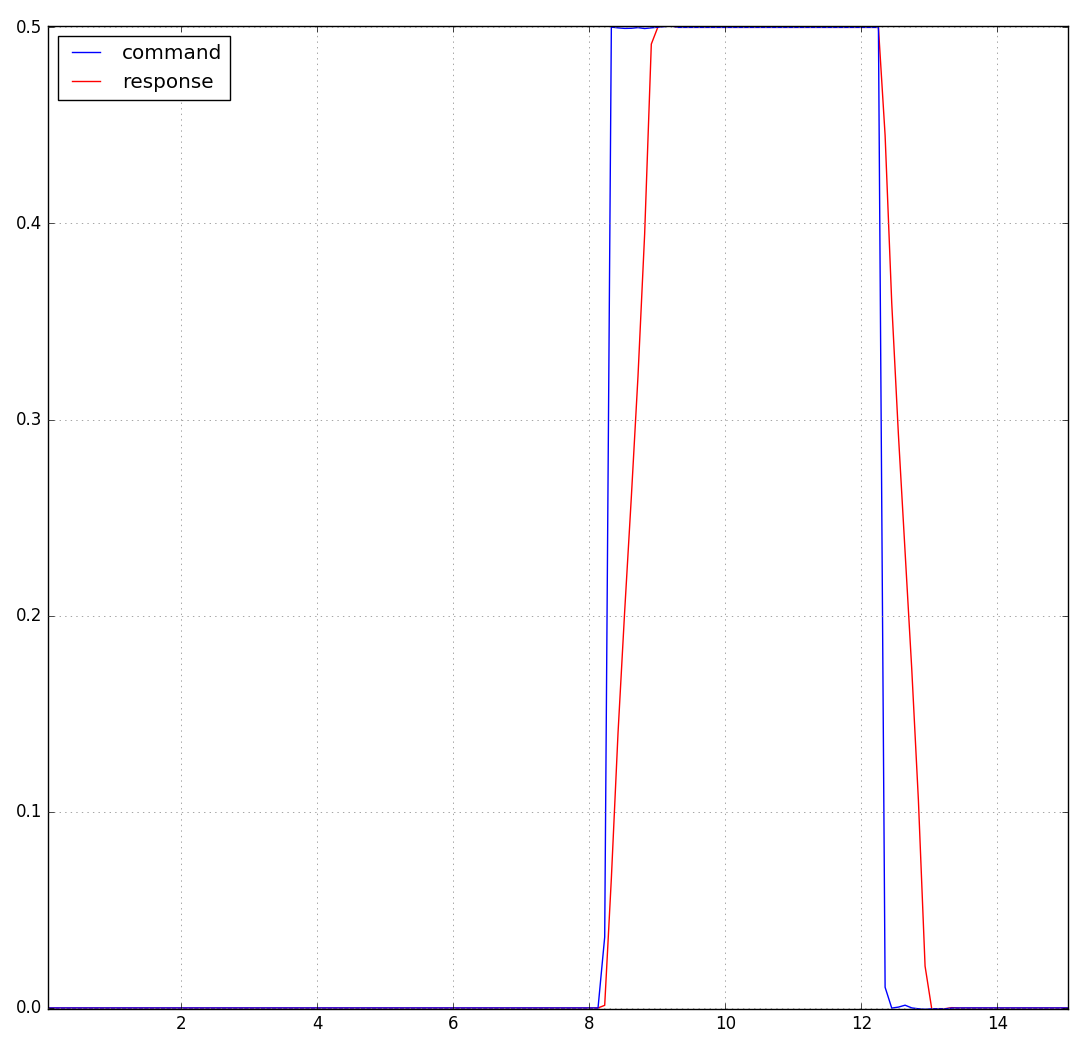
\includegraphics[width=0.7\textwidth]{Figures/90_y.png}
%     \caption{Caption}
%     \label{fig:my_label}
% \end{figure}


%%%%%%%%%%%%%%%%%%%%%%%%%%%%%%%%%%%%%%%%%%%%%%%%%%%%%%%%%%%%%%%%%%%%%%%%%%%%%%%%%%%%%%%%%%%%%%%%%%%%%%%%
%%%%%%%%%%%%%%%%%%%%%%%%%%%%%%%%%%%%%%%%%%%%%%%%%%%%%%%%%%%%%%%%%%%%%%%%%%%%%%%%%%%%%%%%%%%%%%%%%%%%%%%%
\section{Translation with rotation}
For this trajectory, the platform is moving along x direction with constant velocity, and rotate for 360 degree at the same time with the angular velocity as a function of time $\dot{\theta}=\frac{1}{1+exp(t-t_d)}$, where $t_d=5s$ is a delay factor. For this trajectory the ICR is moving around with a relative high velocity and switching between 2 control logic happens twice.
\subsection{Task space velocity response}
\begin{figure}[!h]
    \centering
    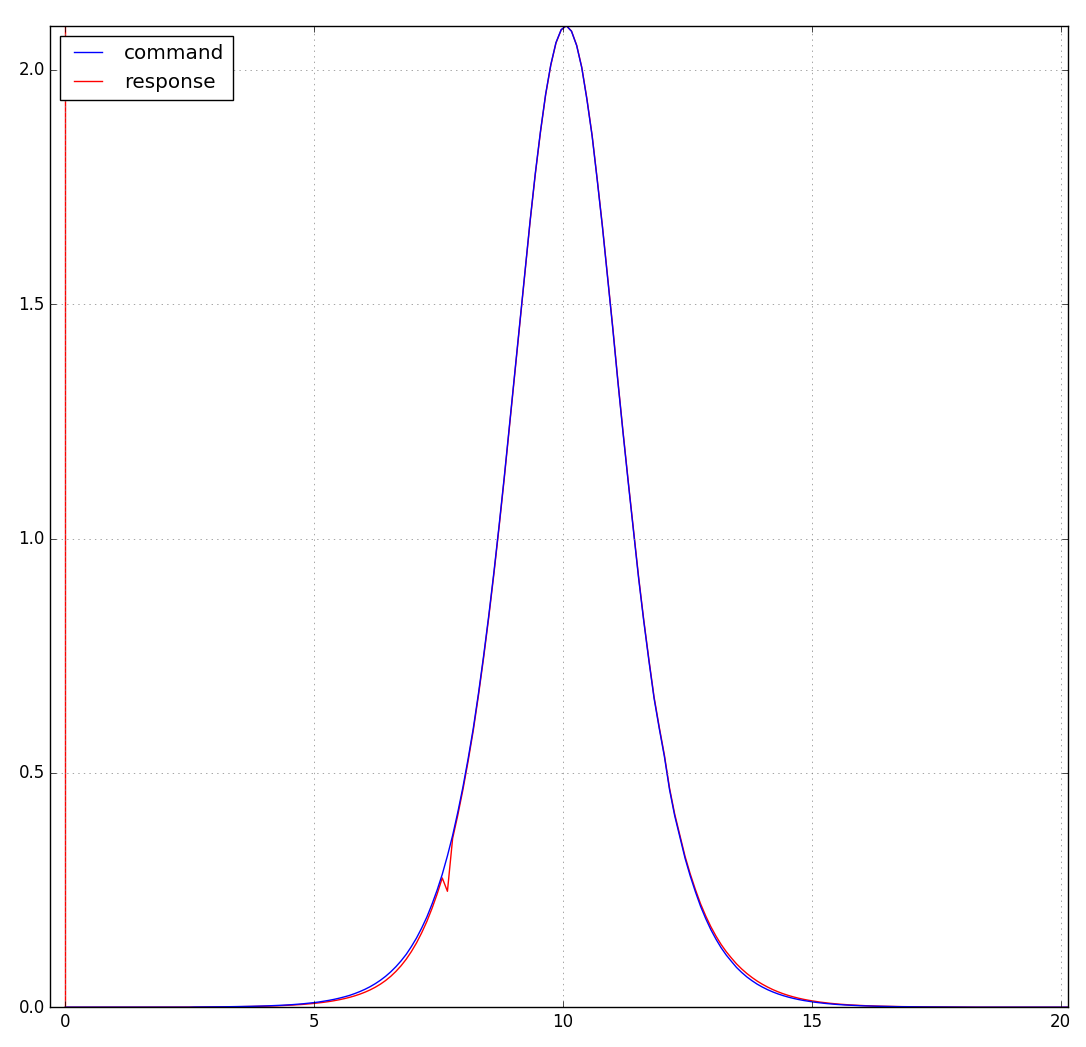
\includegraphics[width=0.8\textwidth]{Figures/360_t.png}
    \caption{$\dot{\theta}$}
    \label{fig:my_label}
\end{figure}

\begin{figure}[!h]
    \centering
    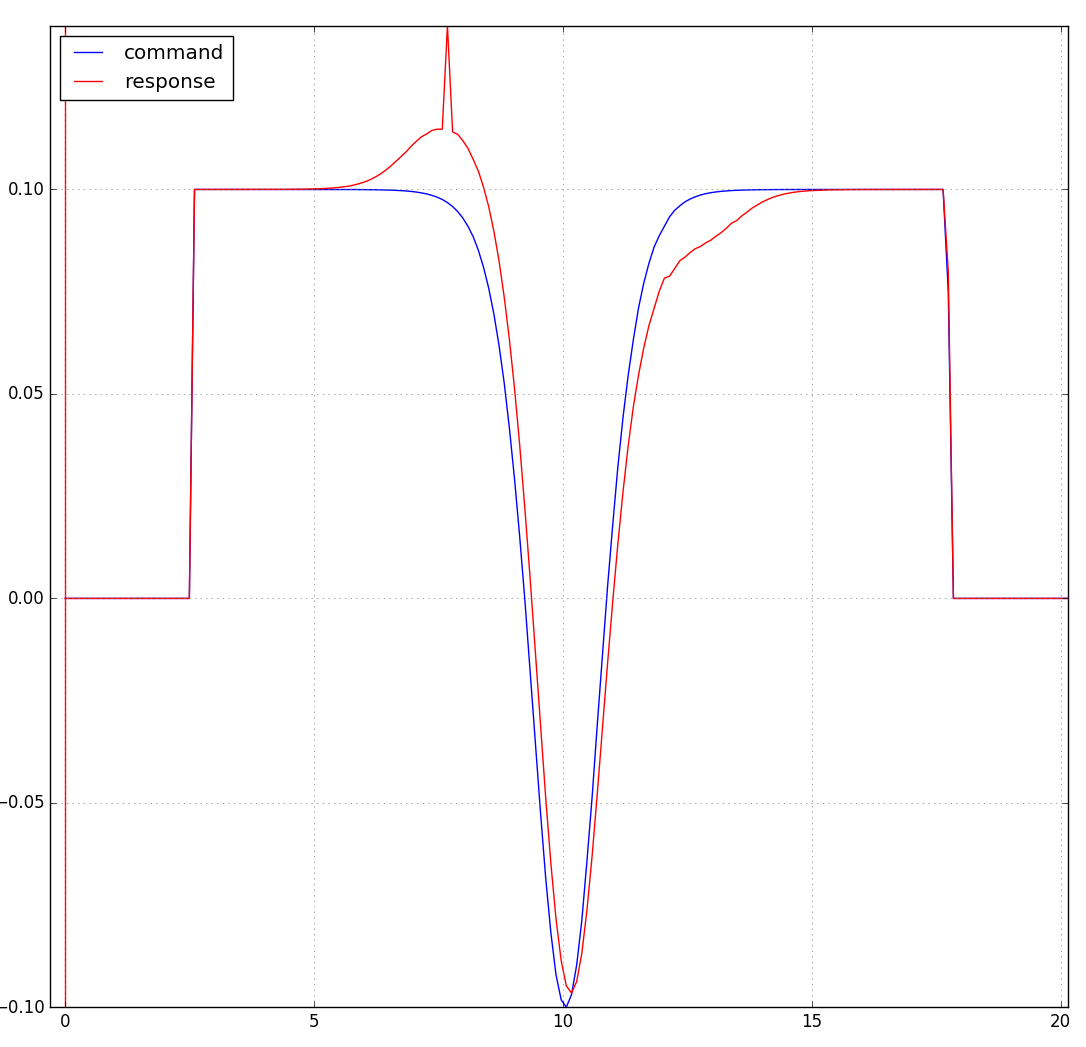
\includegraphics[width=0.8\textwidth]{Figures/360_x.png}
    \caption{$\dot{x}$}
    \label{fig:my_label}
\end{figure}

\begin{figure}[!h]
    \centering
    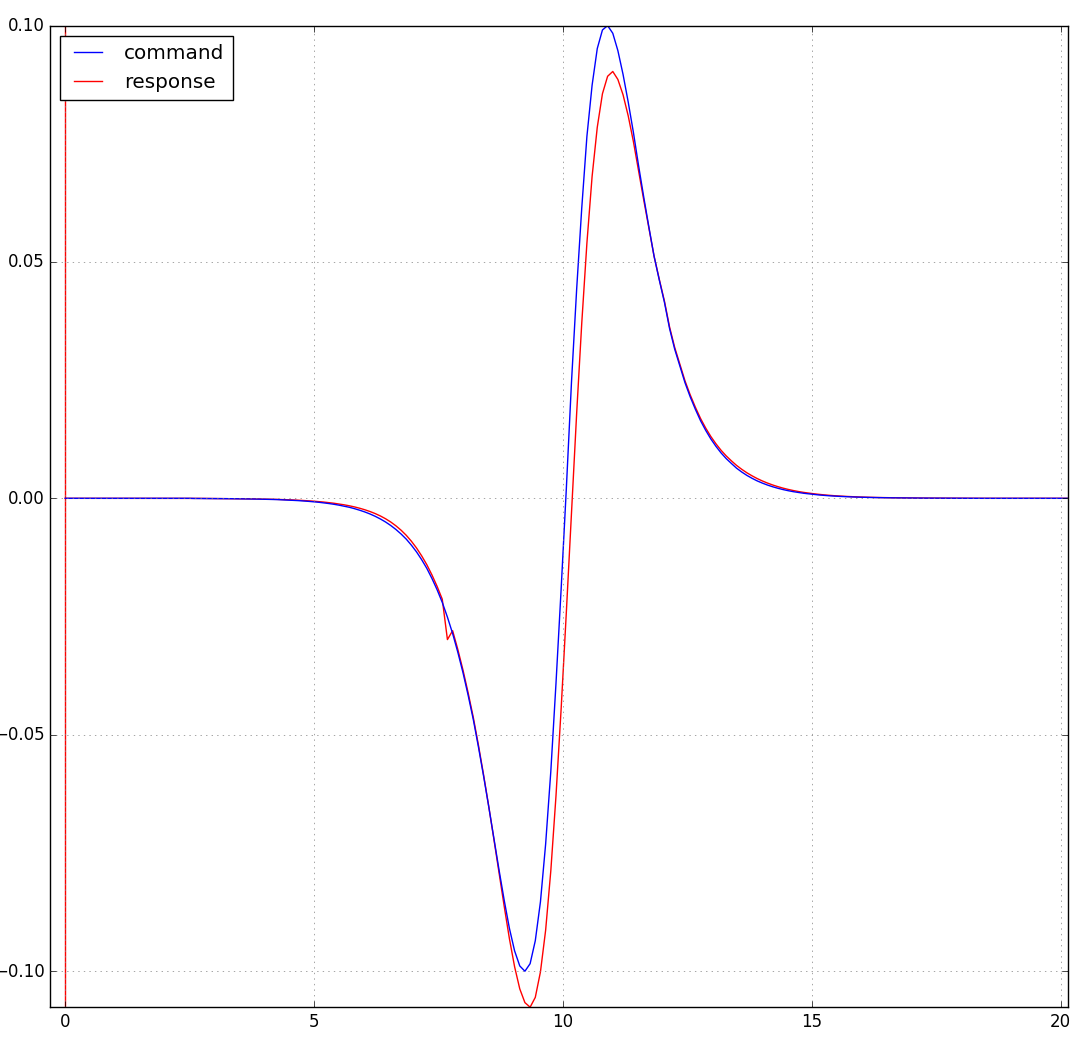
\includegraphics[width=0.8\textwidth]{Figures/360_y.png}
    \caption{$\dot{y}$}
    \label{fig:my_label}
\end{figure}
%%%%%%%%%%%%%%%%%%%%%%%%%%%%%%%%%%%%%%%%%%%%%%%%%%%%%%%%%%%%%%%%%%%%%%%%%%%%%%%%%%%%%%%%%%%%%%%%%%%%%%%%
\subsection{ICR response}

\begin{figure}[!h]
    \centering
    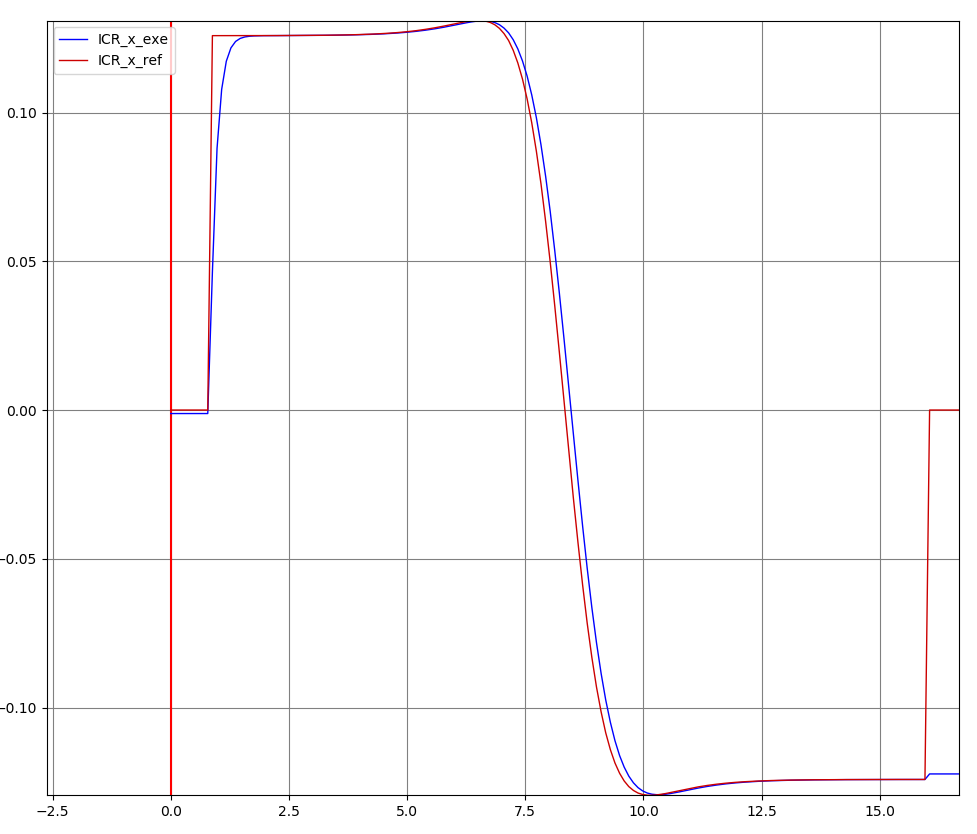
\includegraphics[width=0.8\textwidth]{Figures/360_ICR_x.png}
    \caption{$\Tilde{ICR_x}$}
    \label{fig:360_ICR_x}
\end{figure}

\begin{figure}[!h]
    \centering
    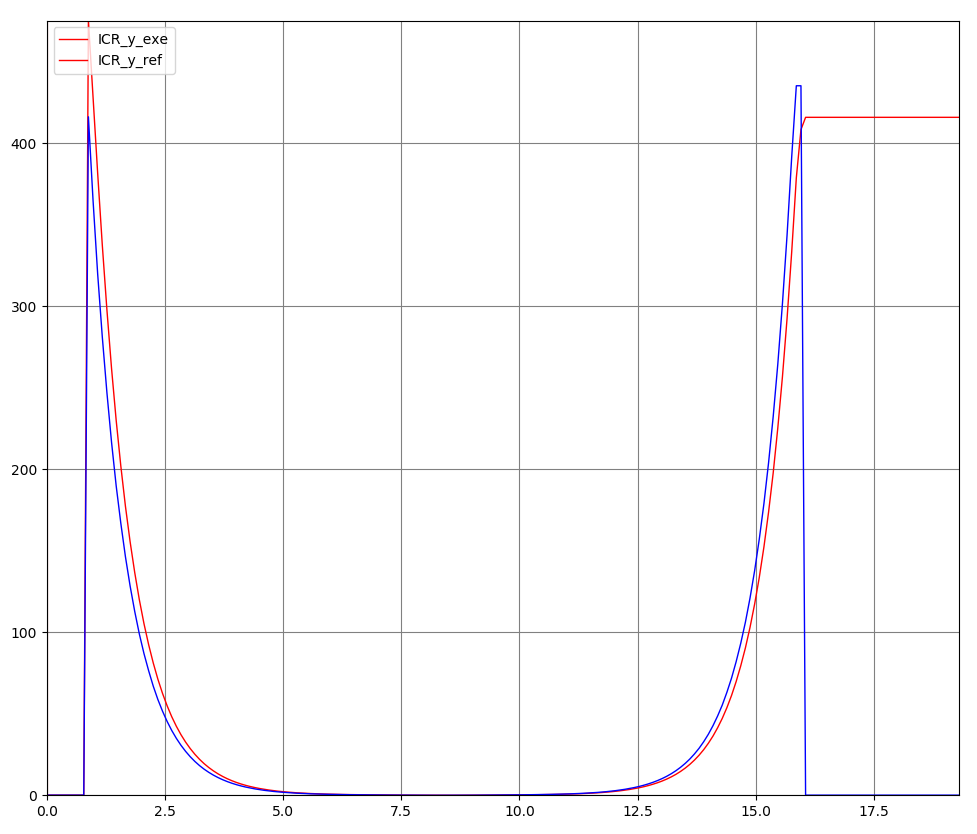
\includegraphics[width=0.8\textwidth]{Figures/360_ICR_y.png}
    \caption{$\Tilde{ICR_y}$}
    \label{fig:360_ICR_y}
\end{figure}
%%%%%%%%%%%%%%%%%%%%%%%%%%%%%%%%%%%%%%%%%%%%%%%%%%%%%%%%%%%%%%%%%
%2345678901234567890123456789012345678901234567890123456789012345
%        1         2         3         4         5         6     
\chapter{Conclusion}
\label{cha:conclusion}

% state problem shortly
Building climate control is important due to provide the optimal conditions, may it be for working inside an office building or for crop growth.
Moreover, building climate control gives the possibility to reduce the costs for operating buildings and to reduce the consumption of energy.

For building climate control the best results are often achieved with nonlinear model predictive control because the climate dynamic is highly complex and nonlinear.
Since obtaining a nonlinear prediction model is an time-consuming task and requires expertise, the work presented an augmented linear model predictive control scheme providing similar results to nonlinear model predictive control.
The error due to neglecting the nonlinear dynamics with a linear prediction model is estimated with Gaussian processes and included in the computations as a parameter.\par\medskip

% contribution
It was shown using the example of a greenhouse that error estimation with Gaussian processes improves the quality for the control significantly.
For set-point tracking the root mean square error was reduced by nearly one order of magnitude.
Applying the augmentation in an economic model predictive control scheme resulted in lower costs for operating the greenhouse while providing better conditions for the crop growth.
Thus, the performance of nonlinear model predictive control and linear model predictive control with error estimation via Gaussian processes are comparable.
Furthermore, the advantages of economic model predictive control were demonstrated.
Controlling the greenhouse climate with economic model predictive control resulted in significant cost savings compared to set-point tracking model predictive control.\par\medskip

% future work
One possible improvement for the by Gaussian processes extended linear model predictive control scheme is the estimation of periodic occurring errors as it was shown in \cite{Klenske.2016}.
Since disturbance variables like the solar radiation are linked to the day-night-cycle a Gaussian process with periodic kernel could model this error.
On-line optimization of the hyperparameters would allow adaption to the current weather situation.

Another direction for further developments is the application of the augmented linear model predictive control scheme on embedded systems.
This is possible due to the low computational requirements compared to nonlinear model predictive control.
For the implementation \textbf{\textmu AO-MPC}, a code generation software package for linear model predictive control, is proposed.
For more details see \cite{Zometa.2013}.

Finally, \cite{Plate.1999} presents a more systematic approach to obtain Gaussian process models.
The influence of all input dimensions and the relations between those can be gradually examined.
By dropping input dimensions and relations with little impact the size of the Gaussian process model is decreased and the interpretability is increased. 
Thus, the computational expense of the Gaussian process models is reduced.

\addtocontents{toc}{\protect\vspace*{\baselineskip}}  % Add some space to the toc

\cleardoublepage              % next content starts on odd page
\listoffigures
%\listoftables

%% BIBLIOGRAPHY %%%%%%%%%%%%%%%%%%%%%%%%%%%%%%%%%%%%%%%%%%%%%%%%%%%%%%%
\bibliographystyle{abbrvnat}
\bibliography{Bibliography/Bibliography_exp}

% \begin{appendix}
% %%%%%%%%%%%%%%%%%%%%%%%%%%%%%%%%%%%%%%%%%%%%%%%%%%%%%%%%%%%%%%%%%
%2345678901234567890123456789012345678901234567890123456789012345
%        1         2         3         4         5         6     
\chapter{Parameters of the greenhouse models}
\label{cha:param_greenhouse}

%\cref{sec:physical_params} gives the physical parameters used in the models.
%\cref{sec:lin_params} gives the point at which the nonlinear model was linearized.

\section{Physical parameters}
\label{sec:physical_params}

\begin{center}
\begin{longtable}{ccc}
		parameter     &   value   &   unit   \\\midrule
		\endhead
		$c_{sph,a}$   &   $1004.5 \cdot 10^3$ & $\unit[]{\nicefrac{J}{kg \cdot K}}$ \\
		$c_{den,a}$   &   $1.2041$            & $\unit[]{\nicefrac{kg}{m^3}}$ \\
		$c_{vol,g}$   &   $2922$              & $\unit[]{m^3}$ \\
		$c_{area,ss}$   &   $877$             & $\unit[]{m^2}$ \\
		$c_{area,p}$   &   $166.8$            & $\unit[]{m^2}$ \\
		$c_{asw,a}$   &   $0.456$            & $\unit[]{-}$ \\
		$V_{tsw,g}$   &   $1.0$            & $\unit[]{-}$ \\
		$c_{cnv,ss-a}$   &   $11.774$            & $\unit[]{\nicefrac{W}{m^2 \cdot K}}$ \\
		$c_{cnd-cnv,a-e}$   &   $14.099$            & $\unit[]{\nicefrac{W}{m^2 \cdot K}}$ \\
		$c_{loss}$      &      $4.2571$         &  $\unit[]{-}$  \\
		$c_{leak}$      &      $0.01$         &  $\unit[]{\nicefrac{m}{s}}$  \\
		$\alpha$   &   $0.0097$            & $\unit[]{-}$ \\
		$\beta$   &   $0.54$            & $\unit[]{-}$ \\
		$R_D$   &   $461.51$            & $\unit[]{\nicefrac{J}{kg \cdot K}}$ \\
		$D_{LAI}$   &   $3.25$            & $\unit[]{-}$ \\
		$MW_{ratio}$ &  $0.622$     &  $\unit[]{-}$ \\
		$p$ & $101325$ & $\unit[]{Pa}$ \\
		$\lambda_v$ & $2.26 \cdot 10^6$ & $\unit[]{\nicefrac{J}{kg}}$ \\
		$c_p$ & $1.006 \cdot 10^3$ & $\unit[]{\nicefrac{J}{kg \cdot K}}$ \\
		$c_{cl,cr}$   &   $0.2$              & $\unit[]{m}$ \\
		$M_{loss,a-e}$   &   $0.2$              & $\unit[]{\nicefrac{kg^2}{m^5 \cdot s}}$ \\\bottomrule
		\caption{Parameters of the greenhouse model}
	  \label{tab:param_greenhouse_model}
\end{longtable}
\end{center}

\section{Parameters for the linearization}
\label{sec:lin_params}

\begin{center}
\begin{longtable}{ccc}
		parameter         &        value           & unit \\\midrule
		$X_{T_{a,a,0}}$   &     $25.0$             & $\unit[]{^\circ C}$ \\
		$X_{H_{a,a,0}}$   &     $0.015$            & $\unit[]{\nicefrac{kg}{m^3}}$ \\
		$U_{ven,0}$         &     $1.0$              & $\unit[]{\%}$ \\
		$U_{shd,0}$         &     $0.0$              & $\unit[]{-}$ \\
		$U_{heat,0}$        &     $0.0$              & $\unit[]{W/m^2}$ \\
		$U_{hum,0}$         &     $0.0$              & $\unit[]{\nicefrac{kg}{m^5 \cdot s}}$ \\\bottomrule
	  \caption{Parameters for the linearization}
	  \label{tab:param_linearization}
\end{longtable}
\end{center}


% %%%%%%%%%%%%%%%%%%%%%%%%%%%%%%%%%%%%%%%%%%%%%%%%%%%%%%%%%%%%%%%%%%
%2345678901234567890123456789012345678901234567890123456789012345
%        1         2         3         4         5         6     
\chapter{Parameters of the Gaussian processes}
\label{cha:param_gaussian_processes}

\section{Set-point tracking}
\label{sec:gp_param_sp}

For two-dimensional wind speed $b_l^a$ and uven und dann squared exponential siehe daaaa.
\begin{table}[h]
	\centering
		\begin{tabular}{c|c}\hline
		bla & bla 
		\end{tabular}
\end{table}

\section{Economic model predictive control}
\label{sec:gp_param_empc}



% \end{appendix}

\end{document}
